\documentclass[12pt]{extbook}

% \usepackage[paperwidth=5.5in, paperheight=8.5in, margin=0.3in]{geometry}
% \usepackage[paperwidth=8.5in, paperheight=11in, margin=0.5in]{geometry}

\usepackage[paperwidth=5.5in, paperheight=8.5in,bindingoffset=0.125in,margin=0.8in]{geometry}

% Fonts and typography

%% Typography
\usepackage[no-math]{fontspec}
\defaultfontfeatures{Mapping = tex-text, Scale = MatchLowercase}

\usepackage{csquotes}

%% Fonts
%\setmainfont{Adobe Garamond Pro}
%\setsansfont{Adobe Garamond Pro}
\setmonofont[Mapping=tex-ansi]{Menlo}

\newfontfamily\coder[Mapping=tex-ansi]{Menlo}

%% Set Sans font in headings
% \usepackage{sectsty}
% \allsectionsfont{\sffamily}

%% Set polyglossia language
\usepackage{polyglossia}
\setdefaultlanguage{english}

% \usepackage[fontsize=16pt]{scrextend}

\usepackage{titlesec}
% \titleformat{\chapter}[display]
%   {\normalfont\sffamily\huge\bfseries\centering}
%   {\chaptertitlename\ \thechapter}{20pt}{\Huge}
\titleformat{\section}
  {\normalfont\sffamily\huge\bfseries\centering}
  {\thesection}{1em}{\Huge}
% \titlespacing*{\chapter}{0pt}{30pt}{20pt}

% \usepackage{titlesec}
% \titleformat{\chapter}[display]
% {\normalfont\huge\bfseries}{\centering\chaptertitlename\ \thechapter}{20pt}{\Huge}


% new page for every chapter
% \newcommand{\sectionbreak}{\clearpage}

% Page

%% Use full page in book style
% \usepackage{fullpage}

\usepackage{fancyhdr}
\pagestyle{fancy}
\fancyhf{}
\fancyhead{}
\fancyfoot{}
\renewcommand{\headrulewidth}{0.1pt}
% \headrulewidth 0.0pt
% \fancyfoot[C]{\thepage}
\fancyfoot[RO, LE] {\thepage}

%% Set line spacing
\usepackage{setspace}
\setstretch{1.2}

%% Disable paragraph indentation
\usepackage{parskip}

\usepackage{afterpage}

\newcommand\blankpage{%
    \null
    \thispagestyle{empty}%
    \addtocounter{page}{-1}%
    \newpage}


%% Start sections from new page
% \let\stdsection\section
% \renewcommand\section{\newpage\stdsection}

\usepackage[labelformat=empty]{caption}

% Images
\usepackage{graphicx}

\usepackage{pdfpages}


\usepackage{xcolor}

%% Tango color scheme
\definecolor{SkyBlue}{HTML}{3465A4}
\definecolor{DarkSkyBlue}{HTML}{204A87}

\definecolor{Plum}{HTML}{75507B}

\definecolor{ScarletRed}{HTML}{CC0000}

\definecolor{Aluminium1}{HTML}{EEEEEC}
\definecolor{Aluminium6}{HTML}{2e3436}

\definecolor{Black}{HTML}{000000}

\definecolor{Grayr}{HTML}{777777}


\usepackage{listings}

\lstdefinelanguage{CODER}{%
  morekeywords = {PAU, JLS, OUIMTQ, ZSMELC, LP, ELJT, L, OLE, ELC, ZRS, XRSP, IRRETUJQ, IRRE, VLXPLMTQ, LTE, XMSLPUQ},
  ndkeywords = {class, export, boolean, throw, implements, import, this},
  % ndkeywordstyle = \color{Aluminium6}\bfseries,
  % identifierstyle = \color{Black},
  sensitive = false,
  comment = [l]{//},
  morecomment = [s]{/*}{*/},
  % commentstyle = \color{Plum}\ttfamily,
  stringstyle = \color{ScarletRed}\ttfamily,
  morestring = [b]',
  morestring = [b]"
}

\lstset{
  language = CODER,
  % backgroundcolor = \color{Aluminium1},
  extendedchars = true,
  basicstyle = \normalsize\ttfamily,
  showstringspaces = false,
  showspaces = false,
  tabsize = 1,
  breaklines = true,
  keywordstyle=\color{Grayr},
  showtabs = false
}

%% Normal enumerates processing
% \usepackage{enumerate}

%% Disable section numbers
% \setcounter{secnumdepth}{0}

\renewcommand\thesection{\arabic{section}}

\begin{document}

  % Title page
  % \thispagestyle{empty}
  % \pagestyle{myheadings}
  % \vspace*{\fill}
  %   \begin{center}
  %     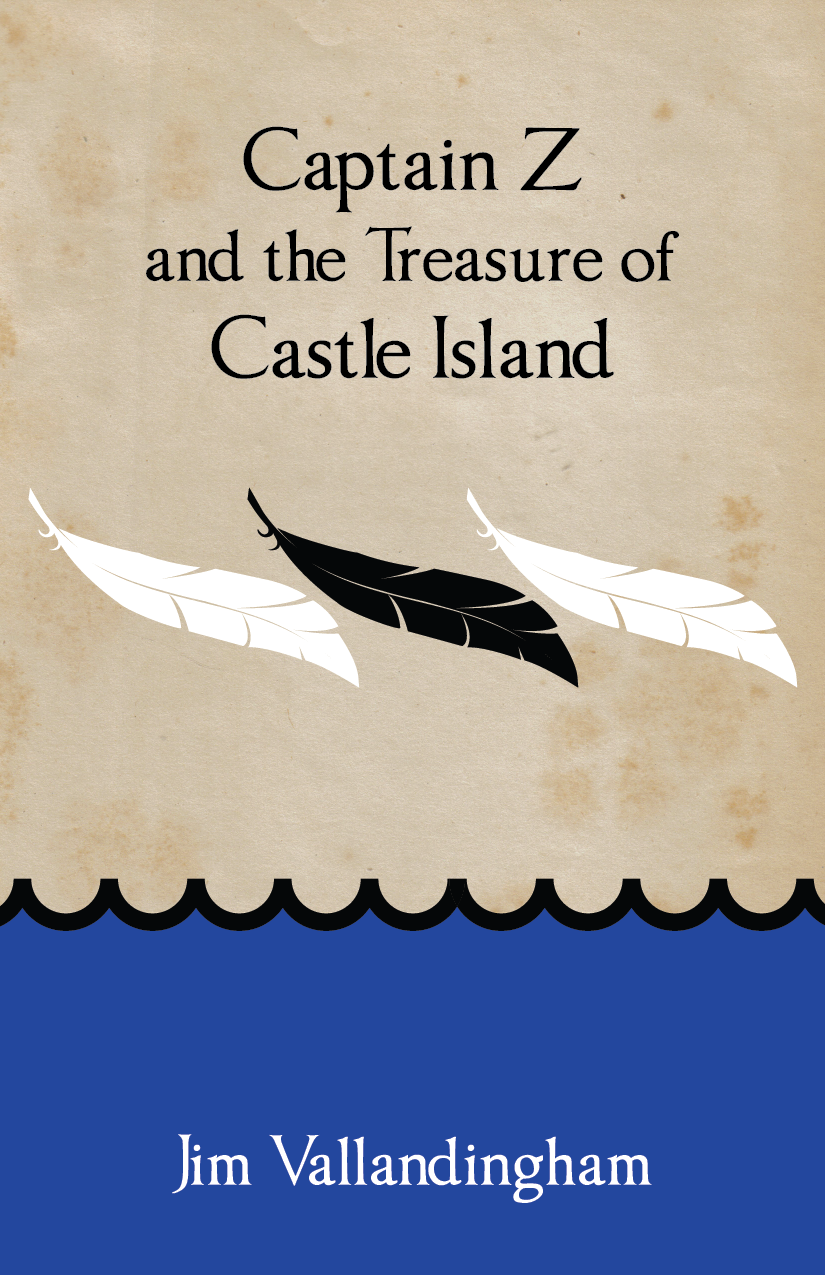
\includegraphics[width=0.98\textwidth]{img/title}
  %   \end{center}
  % \vspace*{\fill}

  % \begin{figure}
  % \noindent\makebox[\textwidth][c]{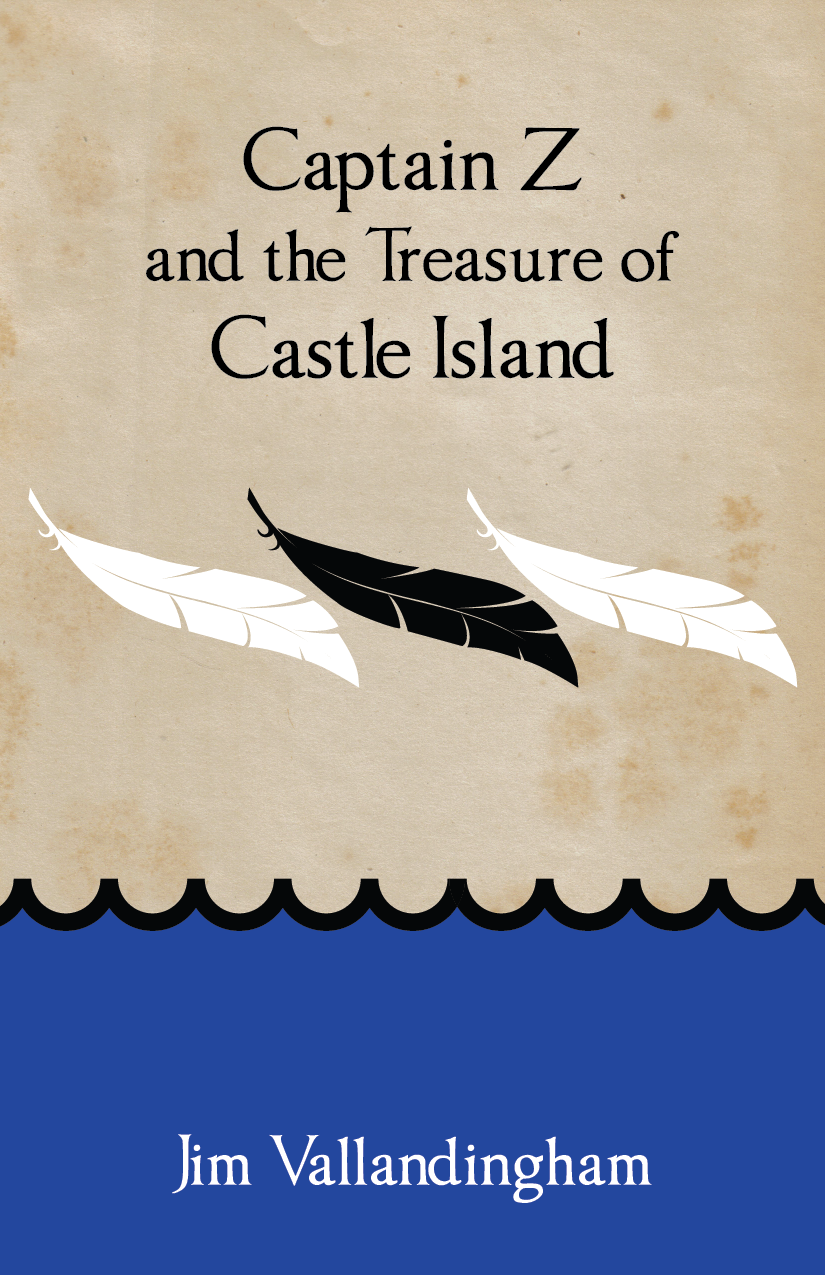
\includegraphics[width=1.4\textwidth]{img/title}}%
  % \end{figure}

  % \includepdf[pages={1}]{img/captain_z_title_2.pdf}

  \pagestyle{empty}
  \vspace*{\fill}
  \begin{center}
  \huge{Captain Z and the Treasure of Castle Island}\\[0.5cm]
  \end{center}
  \vspace*{\fill}
  % \afterpage{\blankpage}
  % \clearpage

  \begin{titlepage}
    \vspace*{\fill}
    \begin{center}
      \huge{Captain Z and the Treasure of Castle Island}\\[0.5cm]
      \large {Jimmy Vallandingham}\\[0.4cm]
      \large {\textit{Illustrated by} Victoria Grace Elliott}\\[0.4cm]
    \end{center}
    \vspace*{\fill}
  % \clearpage
  \end{titlepage}
  
  \begingroup
  \footnotesize
  \parindent 0pt
  \parskip \baselineskip
  \vfill
  Captain Z and the Treasure of Castle Island \\
  Jimmy Vallandingham \\


  Copyright \textcopyright{} 2014 by Jimmy Vallandingham \\
  
  All rights reserved. No part of this publication may be reproduced, stored in a retrieval system, or transmitted in any form or by any means without prior written permission of the copyright owners. 
  
  If you want permission, just let me know.\\
  Contact information can be found at vallandingham.me


  ISBN: 978-1501048449

  First edition: October 2014

  \vfill
  vallandingham.me\\
  captainZbook.com
  \vspace*{2\baselineskip}
  \clearpage
  \endgroup

  \begingroup
  \vspace*{\fill}
  \begin{center}
  To my wife, daughter, and son.
  \end{center}
  \vspace*{\fill}
  \afterpage{\blankpage}
  \endgroup
  \setcounter{page}{0}
  \clearpage
  

  % \frontmatter
  
  \pagestyle{fancy}

  % Book contents
  \section{}\label{section}
  
  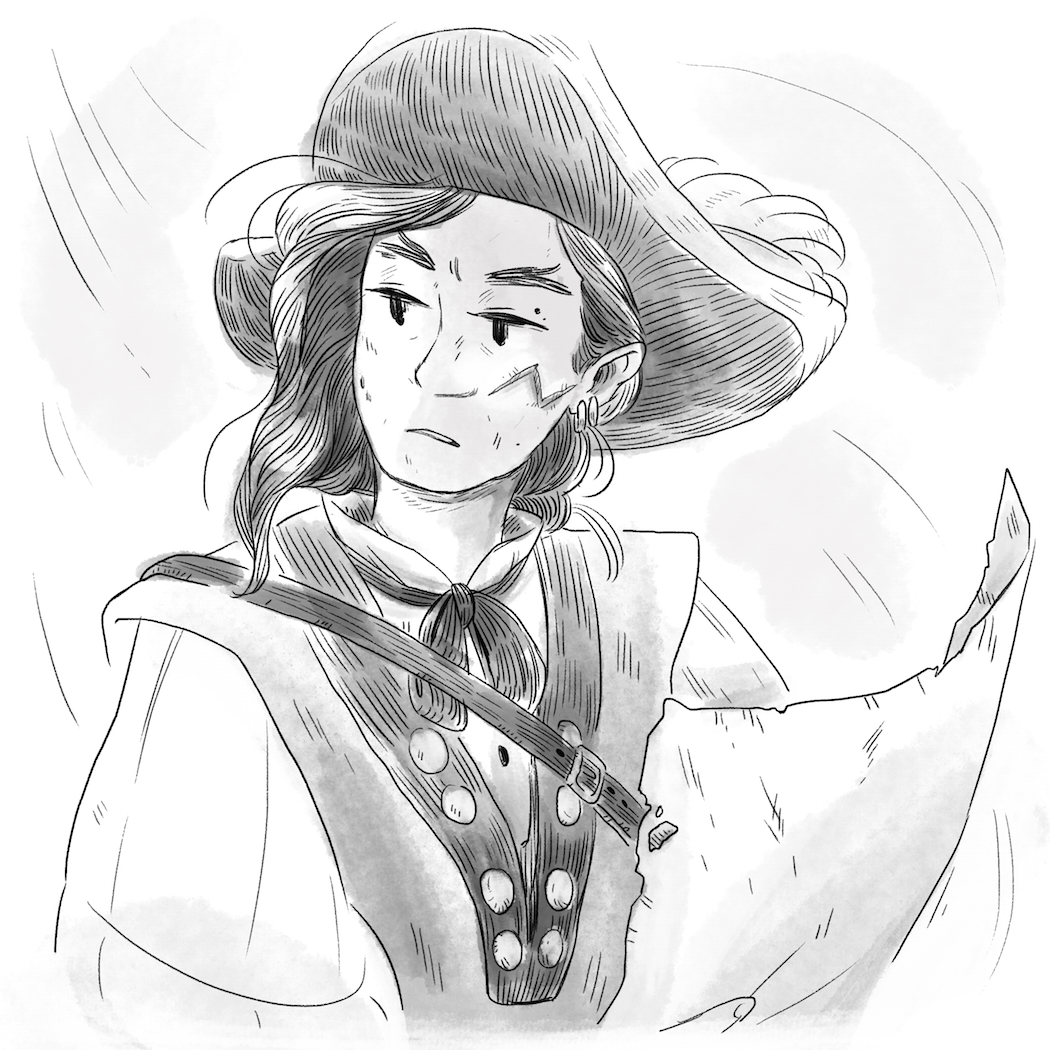
\includegraphics{img/captain_z.png}\\
   Our story begins, as most pirate stories do, in the dark.
  
  The low glow of a lamp, running out of oil, was nearly the only light
  about. The glow of the stars and moon up above helped a bit, but its
  always darkest, as they say, just before the dawn.
  
  The lamp shined its light on a little dirt path that ran between the
  rocks. The path wound its way up through the steep cliffs of a forlorn
  and bare little island. The cliffs, the rocks, the path, and some palm
  trees were about the only things on this island. But this island also
  had something unexpected on it: treasure.
  
  It was because of this treasure that our pirate friend was on this
  little island, in the dark. Though, friend might not be the word to use
  for such a figure as this one.
  
  The little lamp she held gave a glimpse of her face. A jagged scar ran
  across it. Starting at the left ear, it painted a crooked Z across her
  cheek, ending at her nose. She held up a map for a closer look at the
  markings on it.
  
  Her mouth was turned down in a deep frown of concentration. Her eyes
  looked like two pieces of coal, black and smoldering, as they stared
  down at the scrap of paper. This map, she hoped, would soon lead her to
  the treasure that lay hidden on this island. As rare a treasure as
  anyone had ever known, and twice as mysterious.
  
  Assured she was still on the right track, the pirate rolled up the map,
  checked over her shoulder again, and started back up the path.
  
  This is our hero, as it were, Captain Sophia Zephyr, or \emph{Captain
  Z}, as she is known.
  
  But Captain Z doesn't start this tale as a hero. She starts it, as you
  might expect from such a story, as a pirate! An especially crafty
  no-good villain of a pirate.
  
  But, there is a chance she might not stay that way. Yes, there's a
  chance, ever so slim, that she might have a bit of good in her, and that
  good may come out and turn her into a hero.
  
  Will she really turn the corner from villain to hero? Does she have it
  in her?
  
  I don't know. All we can do is watch and listen to find out.
  
  \section{}\label{section-1}
  
  Captain Z stopped for a bit to rest on one of the large rocks along the
  steep path. She checked the map again, making sure she was still on the
  right path, then continued to trudge up the mountain.
  
  The map in her hand was a treasure map of the very island she was on.
  Pirates and fisher folk alike called this place \emph{Castle Island}.
  
  The path she was taking ended at an X on the map, and as you may know,
  an X always marks the spot. And at this particular spot was the treasure
  that Captain Z was hoping to find, and escape with, before she was
  discovered.
  
  You see, Captain Z was not the only pirate creeping about on this island
  in the dark night.
  
  The Dread Captain Spears and his crew of scoundrel pirates were
  searching and scouting the island as well. Except they didn't have a
  treasure map, as Captain Z had stolen it from them. So they were not
  searching for the treasure. Instead, they were searching for her!
  
  \section{}\label{section-2}
  
  Earlier, that same night, things were a different story altogether.
  
  The Dread Captain Spears had the treasure map of Castle Island all
  locked up and safe on his ship the Sea Breaker. At least, he thought it
  was locked up safe.
  
  But he probably wouldn't have thought his map was so secure if he knew
  Captain Zephyr was on her way to take it from him.
  
  The Sea Breaker was moored up a stones throw from Castle Island. Captain
  Spears's plan was for he and his pirate crew to get a good night's
  sleep, and then have the whole next day to search for the treasure shown
  on his map. He had even made his crew go to bed early, much to their
  grumbling and complaining.
  
  But as he and his crew were putting on their pajamas, a little rowboat
  slowly and quietly stole its way toward their mighty pirate ship.
  
  Captain Z was in that little rowboat, along with a hook and rope, her
  lamp, and her feathered hat.
  
  As the sky darkened into night, Captain Z pushed right up to the side of
  the big pirate ship. Swinging her hook around, she threw it up and
  snagged the railing of the ship. Quick as a wink, and quiet as a mouse,
  Captain Z climbed up and was on the top deck.
  
  She tiptoed across the deck, toward the door leading below. Carefully,
  she skipped over squeaky planks and tangles of rope that could trip her
  up.
  
  The door gave a little groan as she opened it, but not one of those
  scoundrel pirates stirred as Sophia slipped below deck.
  
  \section{}\label{section-3}
  
  What a commotion those pirates made while sleeping!
  
  The snoring was so loud that it sounded like a thunderstorm down there.
  
  Captain Z crept past the loud bedrooms and shuffled into the cluttered
  and crowded map room. Maps were everywhere. They covered the tables and
  rolled up and scattered on the floor. Maps stuck out of vases and pots
  and pans. They hung on every inch of the walls, but none of these maps
  was the one Captain Z was looking for.
  
  Over in the corner of the room lay a small wooden chest, no bigger than
  a crab trap. In that chest, Sophia knew, was the one she had been
  looking for. The map that showed the way to the treasure of Castle
  Island.
  
  The chest was locked. Such an important map would be well watched.
  Captain Z knew that the only key to the chest was strung around Captain
  Spears's neck. But there's more than one way to steal a map, and luckily
  for Captain Z, some pirates never think about these other ways.
  
  But she did.
  
  Instead of trying to unlock the chest to get the map, Captain Z just
  grabbed the whole chest, with the map still inside.
  
  Out of the map room and back down the hall went Captain Z and her new
  chest. The chest was heavy, but not too heavy to be carried for a few
  minutes, which is all it would take to get it off the ship. \emph{Yes},
  Captain Z thought, \emph{in a few seconds I'll be off to the island to
  find the treasure, while this crew is still fast asleep in their
  pajamas.}
  
  But while Captain Z was smiling to herself and thinking of how smart she
  was, she forgot to watch where she was going. She reached the steps to
  the deck but missed the first one. Bam! She tripped and the chest came
  crashing down, with her behind it.
  
  All of a sudden the snoring stopped. Out of the bedrooms came shouts.
  
  \enquote{Avast! Who goes there?}
  
  The frightened captain grabbed her stolen chest and flew out of the door
  and on to the main deck, slamming the door behind her.
  
  \section{}\label{section-4}
  
  Captain Z scrambled as fast as she could toward the front of the boat.
  
  The back and forth of the waves and the jumbles of rope nearly made her
  loose her balance as she looked for a place to hide. She had to get out
  of sight before the pirates found her with the stolen chest.
  
  Towards the side of the boat she found a loose tarp covering a few
  crates and barrels. She ducked under the tarp and squeezed herself
  between two of the barrels. Then she held her breath.
  
  Almost immediately, a slew of pirates burst out of the doorway and onto
  the main deck. Still sleepy and confused, they stumbled about looking
  back and forth for whatever could have caused all the ruckus that had
  woken them.
  
  Peeking out of her hiding spot, Captain Z had to cover her mouth to stop
  herself from laughing out loud at the way the sleepy pirates were
  dressed.
  
  They were wearing footie pajamas, like children! The feet on their pj's
  made them slip and slide around on the deck with each wave. The pajamas
  were blue, or green, or pink. And on each of their heads was a little
  sleeping cap with a long tail.
  
  They looked more like baby dolls then terrible pirates!
  
  The biggest of them all, the Dread Captain Spears, finally appeared on
  the deck too, in bright red pajamas. He had ran from his captain's cabin
  in the back of the ship and was still holding one of his cuddly stuffed
  animals. It was a little monkey, one of his favorites.
  
  Hissy, his cat, trotted along beside him.
  
  \section{}\label{section-5}
  
  Now, there are a pages and pages of stories I could tell of the terrible
  Captain Spears.
  
  Everyone and their grandmother knows the story of how Spears, in a rage,
  threw two of his own men overboard just for playing cards. When the were
  dragged back on board, still spitting and sputtering, Captain Spears
  just snarled and said, \enquote{Ye can play when the workin's done.}
  
  \begin{figure}[htbp]
  \centering
  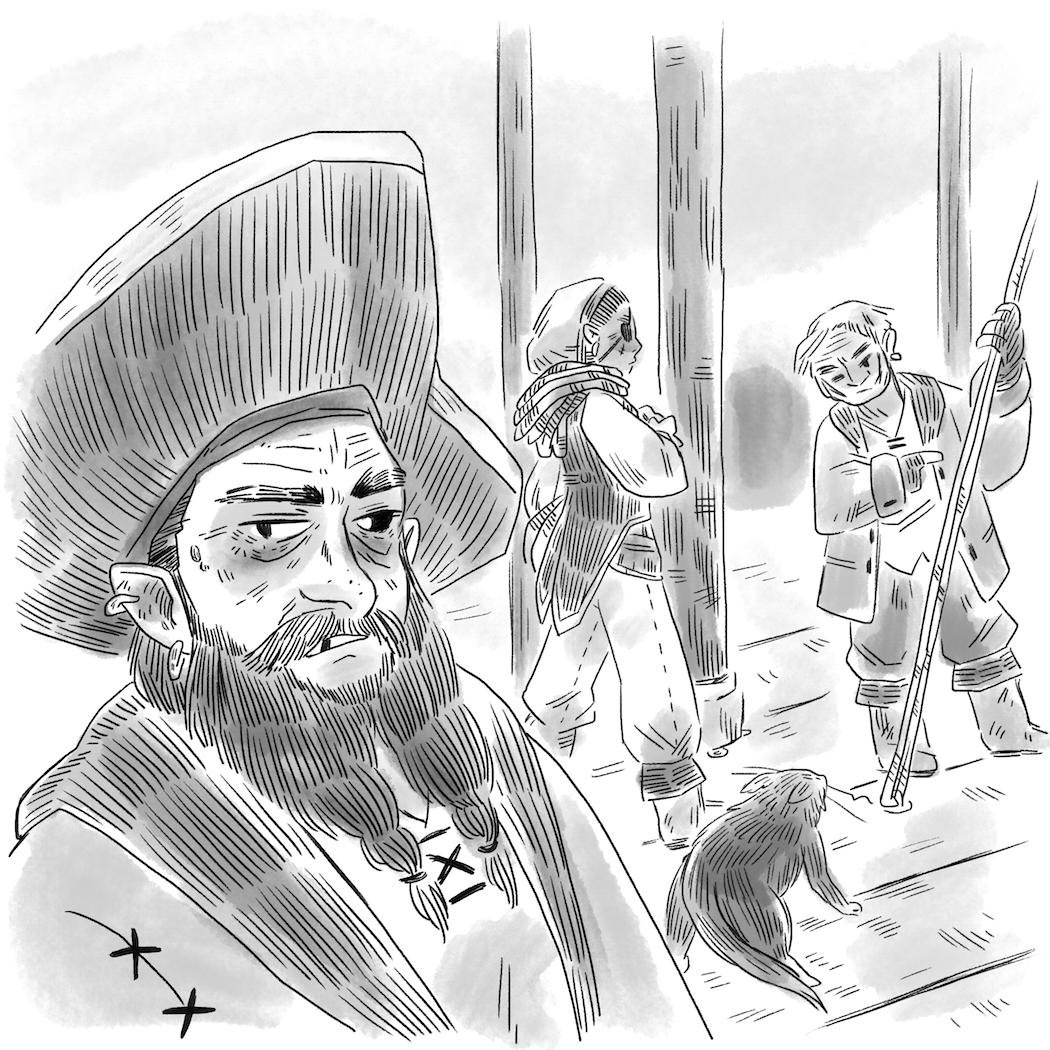
\includegraphics{img/capt_spears.png}
  \caption{}
  \end{figure}
  
  Then, there was the time he poked a hole in another pirates brand new
  hat, just because Spears thought the other pirate looked at him funny.
  
  Or, the time he captured ten dolphins and tied their tails together.
  Then he spent a whole day skiing behind them as they pulled him through
  the water, shouting \enquote{Look at me! King o' the fishes! King o' the
  sea!}
  
  Though I have to hope he knows dolphins aren't fish at all. Sometimes
  pirates aren't the smartest when it comes to that sort of thing.
  
  Of course this is to say nothing of Captain Spears's evil red eye.
  
  Some people said it was a magic eye, and could kill a man with only a
  glare. Others said that Spears was cursed by a foul witch, and the eye
  was markings of that spell. Others said that he couldn't see a wink out
  of it at all, a blindness caused by a run in with a poisonous jellyfish
  when he was just a child.
  
  No one knew who was right or wrong about Captain Spears and his eye. But
  it did seem to glow in the night, like the flame from a candle. And at
  times it changed color, from red to yellow, or even blue.
  
  The eye only added to the fearfulness other pirates felt when they spoke
  of Captain Spears.
  
  For every terrible Captain Spears story, there's a just as terrible a
  story about Hissy, the cat that sailed about with Spears, like one of
  his own pirate crew.
  
  It was said that when Hissy caught mice, it made them walk the plank and
  push them overboard one by one to watch them fall into the water.
  
  Hissy also liked to grab seagulls out of the air as they circled the
  ship. It would rip out all the feathers from the heads of these poor
  birds, and let them go. As such, the only seagulls that still flew
  around the Sea Breaker were completely bald.
  
  The only person that could pet the mean old cat was Captain Spears
  himself. Anyone else who tried would get a scratch and a hiss.
  
  There wasn't a more terrible pirate on the seven seas than the Dread
  Captain Spears. And there wasn't a more frightful cat aboard any ship on
  earth than Hissy.
  
  And both of these villains, as well as a whole crew of scoundrels, were
  now looking for Captain Sophia Zephyr.
  
  \section{}\label{section-6}
  
  Captain Spears's eyes darted back and forth and all around the boat
  looking for something out of place. He had just woken up out of a
  wonderful dream, and his head was still muddled and confused. He hadn't
  yet thought to check the map room to find out if anything was missing.
  
  When Captain Z saw Spears and his cat, she scooted back under the tarp
  as far as she could go. It would be an awful thing to be caught on board
  the Sea Breaker with something belonging to Captain Spears.
  
  She had to escape, but how?
  
  Suddenly, a great commotion broke out. One of the sleepy pirates had
  gotten all tangled up in some of the loose ropes on the deck. While it
  was just rope wrapped around his legs and arms, this pirate thought it
  was the tentacle of a giant octopus up from the depths to drag him into
  the sea!
  
  \enquote{Oh Help! I'm done for! Tis a great Kraken come to swallow me
  whole!} The pirate shouted and flailed his free arm about. His pirate
  companions were slow to help, fearing such a beast could grab them and
  pull them under as well.
  
  When they found this screaming pirate was battling nothing more then a
  piece of rope, they all broke out in laughter (pirates are mean like
  that, always laughing at their mates).
  
  \enquote{Pray, grab my hand and I'll save you from the monster!} one of
  the other pirates called out. The tangled pirate grabbed for a hand, and
  all the others fell to the floor from laughing so hard.
  
  With all this tomfoolery going on, now was the chance for Captain Z to
  escape unnoticed.
  
  She crept out from under the tarp with the chest and headed for the side
  of the ship. Looking over the railing, she saw the little rowboat that
  carried her here still where she had left it, down below.
  
  As she turned back around to check that no one was watching her, she met
  face-to-face with that nastiest of cats, Hissy!
  
  Hissy had jumped up on the railing next to her and stuck its face out to
  scare her. The cat started up a terrible fit of hissing and meowing.
  This startled Captain Z such that she stepped backward, tripped over the
  railing, and went falling head first over the side of the boat.
  
  \section{}\label{section-7}
  
  Captain Z would be dead and drown, her stolen chest lost for certain, if
  it weren't for that great tangle of ropes aboard the Sea Breaker.
  
  The same ropes that had allowed her to escape by tangling up the sleepy
  pirate, had now narrowly saved her life.
  
  As she fell off the side of the ship, some of the rope wrapped around
  her left foot. Now Captain Z was dangling upside-down by her leg twenty
  feet below where she started on the deck, but hanging right above her
  own little rowboat.
  
  What luck!
  
  But time stays still for no man, or woman, as it were. She had to move
  fast to take advantage of that lucky tangle.
  
  Captain Z dropped her stolen chest into the rowboat, which landed with a
  bang. She reached up and unloosed the rope coil around her ankle. Then,
  she dropped down and hit the rowboat with a thud herself.
  
  Sore, but with no bones broken, she put her oars in and started rowing
  as fast as she could.
  
  A few of the pirate crew poked their heads over the railing to look down
  at whatever it was that had just fallen off their boat.
  
  They shouted and waved their arms to bring over the rest of the crew.
  
  Captain Z looked up just in time to see the Dread Captain Spears glaring
  down at her. His red eye blazing like a bright fire, stoked by his
  anger.
  
  He stood there and scowled at her for a time, no doubt trying to figure
  out what to do next. Then he turned and started shouting commands at his
  crew. \enquote{Avast, ya sea dogs! To the aft, double time!} His crew
  all started running to the back of the ship, and disappeared from
  Captain Z's view.
  
  Captain Z focused on her rowing.
  
  The water was too shallow to allow that great giant of a boat, the Sea
  Breaker, to reach her. Instead, they would have to lower their own
  rowboats if they wanted to chase her.
  
  Captain Z cursed her luck and her clumsy feet for such a disastrous get
  away. Still, she had the chest, which meant she had the map.
  
  She had the map, once she got the chest open, that is.
  
  Smiling, Captain Z rowed straight for shore. \emph{There's more then one
  way to open a chest}, she thought again, \emph{and I have the perfect
  key of sorts.}
  
  \section{}\label{section-8}
  
  Back on the deck of the Sea Breaker, Captain Spears and his men were
  racing to their rowboats, which were docked on the tail end of the ship.
  
  Three steps in and two of them had tripped and fallen over even more
  ropes.
  
  \enquote{Blast this darned rope!} Captain Spears yelled. \enquote{One of
  you sea pigs best be cleaning up this mess of a ship.}
  
  \enquote{I'll tend to it right this moment Captain,} one of the pirates
  replied. It was old Jon Thumb, always looking to make things right with
  the boss.
  
  \enquote{Not now, ye meat head,} the captain said. \enquote{We're after
  the intruder.}
  
  The pirates had stopped running to help those that had fallen back on
  their feet. Sally Snake Eye stood there with a confused look on her
  face.
  
  \enquote{But captain, why was our intruder\ldots{} intruden?} She asked.
  
  It was a good question. Captain Spears just stood there scratching his
  beard. His red eye now a pale purple hue. Truth be told, he didn't know
  what Captain Zephyr had been doing on his ship. With all the commotion,
  he had forgotten to think.
  
  But thinking now, he knew that her being there was certainly nothing but
  trouble for him. But what kind of trouble, exactly?
  
  \enquote{Me thinks she be spying on us whilst we sleep,} Golden George
  offered as an answer.
  
  \enquote{You always be thinking someones wanting to spy on you,}
  responded Captain Spears. \enquote{Ain't no one wants to see your ugly
  face. Be it awake or sleeping.}
  
  Golden George felt hurt and put on a sour face. \emph{Plenty of people
  liked the look of me}, he thought. \emph{Spears is just jealous.}
  
  \enquote{Perhaps she was in the kitchen, stealing our grub,} another
  pirate suggested.
  
  \enquote{Perhaps she be stealing our gold. Though she found that we
  ain't got any, and left.}
  
  \enquote{Mayhap she came to steal your cuddly toys.}
  
  That last remark came from Barnacle Bill. He got an elbow and a shush
  from Sally Snake Eye. Talk of Captain Spears's stuffed animals always
  ended in nothing but shouting and kicking from Spears. His crew weren't
  supposed to know about his embarrassing collection, though it wasn't a
  secret to anyone.
  
  Everyone looked at Captain Spears. He was getting mad alright. Lucky for
  Bill though, not because of the mention of his cuddly animals. He was
  thinking about Captain Zephyr, and his eye went from purple to a bright
  hot red.
  
  \emph{Sophia Zephyr was there to steal something, alright}, he thought.
  But it wasn't food, nor gold, nor his cuddly monkey. But what? The
  thought was almost in his head.
  
  \enquote{The map!} He cried, turning around with a twirl. He shot out
  like a bullet toward the map room. His scoundrel crew followed along at
  his heels.
  
  \section{}\label{section-9}
  
  \emph{The map is safe, I've got the key. The map is safe, I've got the
  key.} This is what Spears told himself as he hustled down the stairs
  towards the map room.
  
  The only key to the chest where the map was stored was still wrapped
  around his neck. He could feel it swinging back and forth as he ran.
  
  He burst into the map room. Looking at the corner where the chest should
  be, he let out a groan.
  
  \enquote{She's grabbed the map, chest and all!}
  
  \enquote{But Captain. It still be locked,} Golden George said. He was
  most likely right, but no one would steal a chest without an idea of how
  to open it. Captain Spears knew that much.
  
  \enquote{Blast that Zephyr,} Spears sputtered. \enquote{Let's get to
  rowing. We'll track her down on the island.}
  
  \enquote{In the dark?} Asked Barnacle Bill, looking a bit sheepish and
  scared.
  
  \enquote{The dark matters not. What matters is the treasure,} Captain
  Spears replied. \enquote{She has the map which means no treasure for us
  unless we get it back, savvy?}
  
  Captain Spears was also thinking of the other piece of paper in that
  stolen chest. The message. He was certainly a fool to keep that letter.
  A fool to even open it up and read it. But read it he had.
  
  There was a chance she would never crack the code, leaving the plans a
  secret. Yes, there was that chance, but knowing that wily Captain
  Zephyr, it was a small chance indeed.
  
  Captain Spears needed that letter and the map before everything was
  ruined. He couldn't bear to think of the trouble he'd be in if it was
  found he let it all get stolen. Just the idea sent shivers down his
  back.
  
  \section{}\label{section-10}
  
  \begin{figure}[htbp]
  \centering
  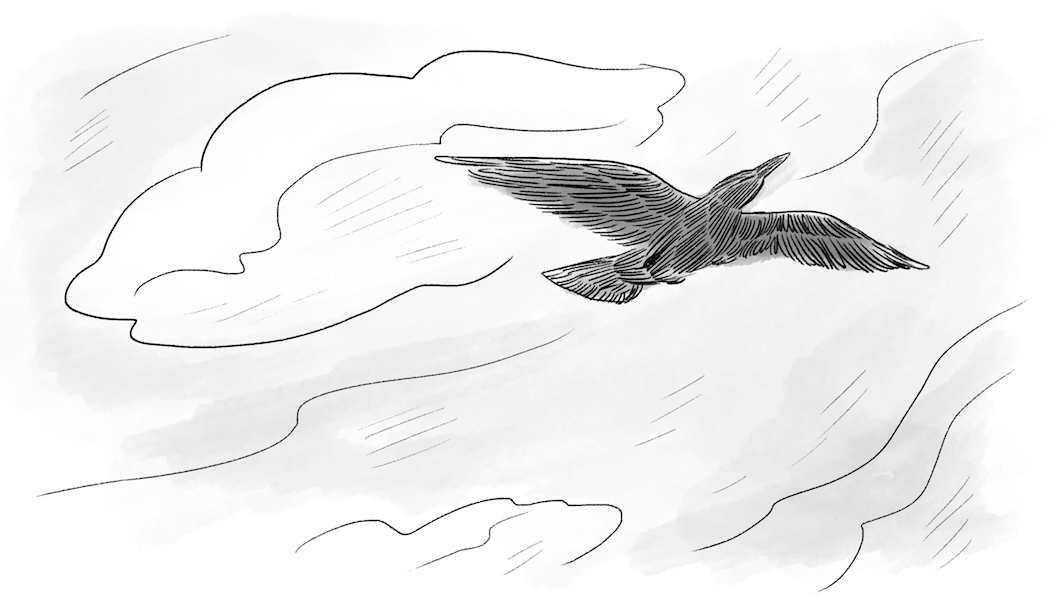
\includegraphics{img/muddle.png}
  \caption{}
  \end{figure}
  
  The rowboat skidded into the shallow water near the beach. Jumping out
  into the shallows, Captain Z pulled the little boat up on the shore.
  
  Her arms were tired and sore from all that rowing. She grabbed the chest
  from the boat and dragged it up the beach.
  
  She made it to the first palm tree that was growing out on the beach,
  then she turned around and gave a little whistle and two clicks.
  
  Out of the black sky swooped a big black bird. It cawed as it flew up to
  the palm tree. It perched in the tree and peered down at the chest in
  Captain Z's hands.
  
  This was Muddle, the crow. Captain Z's friend and companion.
  
  Some pirates have parrots. Others cats, or rats, or dogs. Captain Sophia
  Zephyr was partial to crows, and to Muddle in particular.
  
  Captain Z had rescued the crow when it was just a baby. Blown out to sea
  and tossed among the waves, Captain Z had found the little Muddle in an
  empty bread basket. She raised her on fish, clams, and shrimp, and had
  taught it all manner of tricks and skills.
  
  The name Muddle came from the crows bad luck. It just as often messed
  things up as make them better, but Captain Z loved her just the same.
  
  And at this moment, Muddle was needed quick. She was the key to opening
  the chest.
  
  Captain Z left the chest on the sandy beach. She called up to the crow.
  \enquote{Away to it Muddle. Crack that lock.}
  
  The big bird knew what those words meant. She flew down to the ground
  and hopped over to the chest. Cocking her head to one side, she looked
  up and down and all over the chest. Then she gave another caw.
  
  Off Muddle went into the night. Flapping slow and low to the ground,
  flying around the trees near the beach. Here and there she stopped and
  picked up something off the ground. When she returned, her beak was full
  of sticks that she dropped in front of the chest.
  
  Some of the sticks were short, some long, some fat, and some skinny.
  Muddle eyed the lock on the chest again and then grabbed one of the
  shorter fatter sticks and went to work.
  
  Up she flapped to perch on the top of the little chest, holding the
  stick in her beak. Then, she stuck the stick into the keyhole along with
  the tip of one of her claws.
  
  In the dark, it was hard to see what was going on, but after a moment or
  two there was a soft click noise. Muddle had unlocked the chest.
  
  \section{}\label{section-11}
  
  Smiling, Captain Z brought out a piece of clam from her pocket.
  \enquote{Good work my pretty bird,} she said as she threw her the clam.
  Muddle flew up to perch on a palm tree to enjoy her treat.
  
  Captain Z turned back to the chest. She lifted its lid up. The chest
  opened with a creak. Captain Z quickly looked up and down the beach to
  check for trouble, then brought her lamp in close.
  
  Even for such a small chest, there wasn't much inside it. Captain Z only
  saw the map, rolled up and tied with a bow. Seeing this bit of paper
  took her breath away. Finally she had a way to the treasure on this
  fabled island.
  
  Carefully she picked the map up, untied it, and rolled it out on the
  sand.
  
  In the low lamp light it was hard to make out the words, but that was
  Castle Island all right. The very island she was on now. The very island
  she had searched three years to find. The cliffs on the map were the
  same shape as the cliffs she could see, just barely, down the beach.
  Their jagged edges cutting across the paper and the dark sky.
  
  The markings on the map showed a path that led up into those cliffs. A
  path where, at its end, Captain Z would have her treasure.
  
  Time to start the search, she thought to herself. Captain Z got up, and
  dusted the sand from her knees. She was just about to start off toward
  the cliffs when Muddle gave a puzzled squawk from above.
  
  Captain Z looked up at Muddle, then back down at the chest. There was
  something else inside.
  
  Bringing the lamp in close again, she looked inside and pulled out a
  small yellow envelope with a piece of paper inside.
  
  She opened the envelope and unfolded the paper.
  
  On it, was written a whole jumbled mess of letters. Captain Z couldn't
  make heads or tails of it. Were these words? Did it say something? Where
  was the start? Where was the end?
  
  Why would such a mess of letters be so important to Captain Spears that
  he would want it locked up?
  
  Such questions, that didn't concern the treasure on Castle Island were
  best held for another time. Captain Z folded the paper and put it back
  in the envelope. Then she put that envelope in a small pocket on the
  inside of her vest.
  
  \emph{That should keep it safe till there's more time,} she thought.
  \emph{Right now, I need to find that path.}
  
  \section{}\label{section-12}
  
  She blew out the flame of her lamp and headed up the beach toward the
  cliffs. Muddle followed, silently flying above.
  
  The other pirates might be close now, so she needed to make sure to keep
  hidden and stay in the dark.
  
  The cliffs loomed high above as she got closer. If you squinted, you
  could probably imagine why someone thought to name the place Castle
  Island. But to Captain Z, the cliffs looked more like the tallest fence
  in the world, covered with spikes, and impossible to climb.
  
  And yet, there was a way up. There had to be. A hidden path through
  those sharp rocks. She just had to find it, and that is why she needed
  the map. For, at the end of that path was a treasure more wonderful then
  you could ever imagine.
  
  Well, at least that was what Captain Z hoped for, what she had heard,
  and what she had told herself.
  
  Truth be known, she didn't really know what was waiting at the end of
  that path to be found. In fact no one alive really knew the truth of the
  treasure of Castle Island.
  
  \section{}\label{section-13}
  
  Three years ago, almost to the day, Captain Z had first heard the tale
  of the mysterious island and its wondrous hidden treasure.
  
  The storyteller had been another pirate, the friendly Sammy Two Toes.
  Sammy had told such a tale that Captain Z knew she would have to find
  the treasure someday.
  
  At that time, Captain Z was no captain at all, as she had no boat of her
  own. She was just one of the crew of the Wind Breaker, charged with
  swabbing the deck and polishing brass. But that didn't stop Sophia
  Zephyr from dreaming and plotting. All things change with the times and
  the tides, as they say.
  
  By and by, Sophia Zephyr became Captain Z and took control of Wind
  Drinker. But this is a tale for another time. By then, she had heard the
  story of Castle Island a hundred times or more. And each time, it ended
  with a different surprise. A different guess at the treasure to be
  found.
  
  Some, like Sammy Two Toes, said it to be a huge diamond. As large as
  your fist, and as heavy as your head. Sammy had said it shone brighter
  then the sun.
  
  But other folks had different ideas about what was hidden there. Some
  said gold or jewels. Others said magical bells, wands, or books. One old
  man even thought there to be a room full of the tastiest meats and pies
  ever to be found. Never mind how such a room could be kept stocked with
  such treats, or why this food would be on an island with no one to eat
  it.
  
  Captain Z didn't know which of the stories to believe, but she knew
  Castle Island held something worth searching for. And that's why she
  kept searching for a way to find the island and a way to find the
  treasure hidden there.
  
  \section{}\label{section-14}
  
  \begin{figure}[htbp]
  \centering
  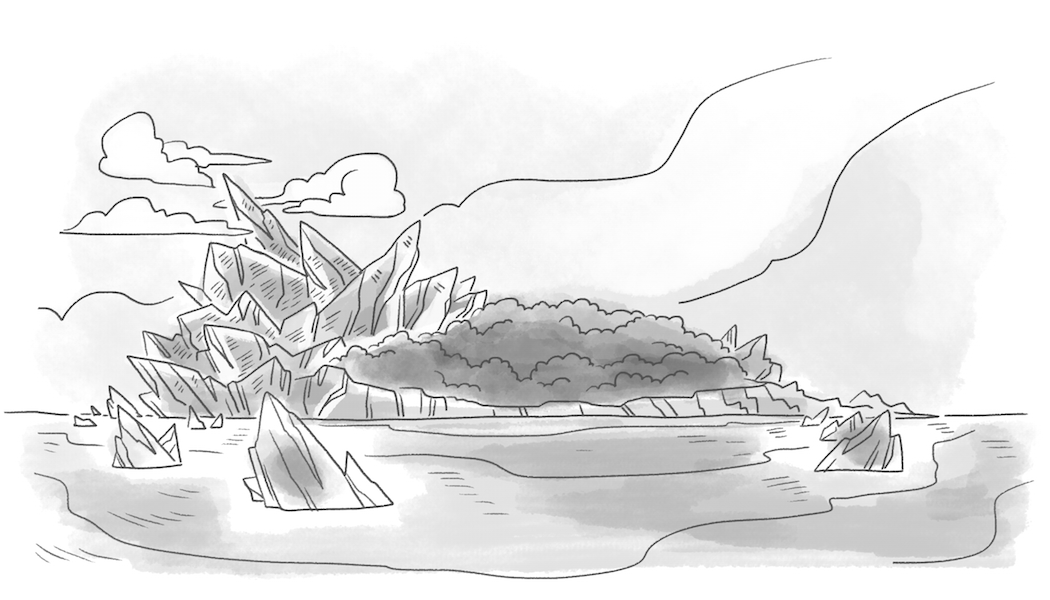
\includegraphics{img/castle_island.png}
  \caption{}
  \end{figure}
  
  Now Sophia had finally found the island, and was close to finding the
  treasure. But she had to move fast, else all might be lost.
  
  Captain Z was at the base of the cliffs, looking back and forth in the
  dark for a path. The cliffs were so steep at the bottom that no one
  would be able to climb them.
  
  Though she looked all around, she could see nothing that resembled the
  start of a path.
  
  \emph{Well, it wouldn't have been lost for so long if I were able to
  find it too easily}, she thought.
  
  She ducked behind one of the many big rocks about, and lit her lamp
  again to take a closer look at the map.
  
  On the map, there was a little arrow that pointed at the base of the
  cliffs. Next to the arrow, three triangles were drawn. Under them were
  the words \emph{Demon's Hand}.
  
  Captain Z looked up again and walked further away from the beach. She
  hoped the trees and bushes here kept her lamp hidden from watching eyes
  along the shore.
  
  She walked along the rocky steep side of the cliffs. It was slow going.
  
  Large rocks and boulders were everywhere. More then a few times, the way
  was blocked by one of these big rocks and she had to backtrack to find
  another way around.
  
  Walking alongside one of these boulders, a root caught her foot and sent
  her sprawling to the ground.
  
  She crawled to her knees and sat down. Her leg hurt now from the fall
  and her arms were still sore from the rowing and scratched from the
  bushes and trees. She had the feeling of wanting to just give up and row
  away. Maybe the treasure wasn't even here anymore. Maybe the whole story
  was made up.
  
  Sitting on the ground with these thoughts in her head, she finally
  looked up to see what was around her. The moon shine down to light the
  cliff walls. Something there made her heart skip a beat.
  
  In fact it was three somethings. Three big rocks broke out of the
  ground, bent and pointed like claws. Here was the spot on the map that
  she had been looking for!
  
  She jumped up and ran as fast as she could to the three big stones.
  
  At first, it didn't look like any path started here. The cliffs were
  just as high as anywhere else. But when she squeezed her head behind the
  claw closest to the cliffs she saw a crack in the rocks. You wouldn't
  see it if you didn't know where to look, but there it was, a path up the
  cliffs.
  
  Captain Z squeezed her arms in past the rock and then pulled the rest of
  herself into the crack.
  
  She could see the path heading up the cliffs, zig-zagging right up the
  side.
  
  Captain Z started walking quickly up the path, excited to be so close
  now, but on the look out for more roots on the ground and pirates
  behind.
  
  \section{}\label{section-15}
  
  Now we find Captain Z in the same spot in the story as where we started.
  Though now we know a great deal more about the where and the why of what
  she is doing.
  
  Captain Spears and his men are rowing fast to reach the island and start
  the search for the pirate thief.
  
  Captain Z is well on her way to finding out what secrets Castle Island
  really hold.
  
  And now there is this mysterious note with its jumble of letters. It
  belonged to Captain Spears. Now it is in the pocket of Captain Zephyr.
  But as to what it said, or who it was from, we have no idea.
  
  Will Captain Spears find our hero, Captain Z?
  
  Will Captain Z find the treasure and escape?
  
  I don't know. All we can do is keep reading, and hope against hope that
  everything will turn out alright.
  
  \section{}\label{section-16}
  
  Captain Z was halfway up the giant of a hill when dawn started to break
  in the Eastern sky. She was on the wrong side of the cliffs to see the
  water or the sun rising up from them, but a pink light started to glow
  around the cliffs.
  
  Daylight would make finding the treasure easier. It would make Captain
  Spears's job of finding her easier as well. Captain Z pressed onward and
  upward.
  
  At the fork in the path, the map showed that left was the direction to
  take. Then the trail should curve back to the right before more
  zig-zagging up a steeper part near the top. Captain Z had already run
  into more then a few dead-ends and wrong turns. It's hard work to read a
  treasure map, especially in the dark. But she was determined not to
  quit. She was too close to the treasure now.
  
  Captain Spears and his scoundrels were still nowhere to be seen. She
  figured they should be on the island now. She hoped that there was not
  another way up the cliffs that wasn't shown on the map. It would be a
  terrible surprise to reach the X on the map and have Spears and his crew
  waiting there for her.
  
  With the pink light over the hill above her, she picked up the pace and
  started to jog up the path. \emph{Even if he is there waiting,} she
  thought, \emph{I'll still be the one leaving this island with the
  treasure. Someway, somehow, I will be the one.}
  
  \section{}\label{section-17}
  
  Captain Spears peered out into the night as his men rowed them toward
  the shore. \emph{At least this eye is good for something,} he thought,
  looking out into the dark. Though it was night time, to Spears,
  everything was brightened through his glowing eye. The world looked as
  if the sun was still up, but hidden behind a cloud.
  
  The eye also allowed him to see things that were far away as if they
  were closer, like a spy glass. Captain Spears scanned the island off in
  the distance, looking for signs of Captain Z. There on the beach, he
  could see her empty rowboat on the sand. That meant she had already made
  it on the island and was looking for the treasure.
  
  His eye followed the beach up toward the cliffs at the North end of the
  island. He looked for her there among the rocks and trees, but saw
  nothing.
  
  Then, high above the cliffs, Spears's red eye caught sight of a big
  black bird floating lazily on the updrafts. \emph{That could only be
  Zephyr's crow,} he thought. \emph{That thing always gives her away.}
  
  \enquote{We'll land up there,} he said to his men while pointing. The
  spot was up the beach, close to the cliffs.
  
  They made it to shore and pulled their rowboats up on the sand. Then
  they set off creeping along the coast, heading for the cliffs.
  
  Captain Spears was leading the group. That red eye of his guiding him
  through the dark. The eye brought the ground closer, as if he were down
  there on his hands and knees with his nose to the sand like a
  bloodhound.
  
  Spears could see the little scuffs in the sand made by the footsteps of
  Captain Zephyr as she walked the beach not more than an hour ago. A
  normal eye would miss these scuffs. But the red eye saw this, and a
  great many other things. Captain Spears tracked Sophia up the beach and
  around the cliffs. His men followed.
  
  They reached the three jagged rocks, and Spears knew they were close. He
  had looked at the map for a bit while he had it. He remembered the
  drawings of the rocks and where the path was supposed to be.
  
  The scoundrel pirates followed their captain down to the claw's furthest
  finger. They were amazed when he showed them the secret path behind it.
  
  \enquote{This way, ya mutts,} he growled as he smiled. \enquote{She'll
  be leading us to the treasure, by and by.}
  
  \section{}\label{section-18}
  
  At the top of the cliffs, Captain Z opened the map again. It showed a
  hole among the rocks. A hole that led down into a little cave. And in
  that cave, the X was marked, the spot where the treasure lay. But this
  hole leading to the cave was covered and hidden.
  
  The map showed a scrawny, spindly pine tree, next to a wide rock. Under
  that rock was supposed to be the hole. She hoped that the tree was still
  alive and hadn't been knocked down by a storm. The winds could blow a
  gale out here in the ocean.
  
  Captain Z scouted around along the top of the cliffs, being careful with
  her feet along the edge. Looking down, it was a long drop to the ocean
  below. One wrong step and\ldots{} well she rather not ponder the result.
  
  Finally, after almost an hour atop the cliffs looking for the tree and
  the rock, she found them. The tree was down at the bottom of a little
  hill, right at the edge of the cliffs. It looked just as scrawny and
  spindly as it was drawn on the map.
  
  The wide rock next to it was covered with dirt, a bit of grass, and pine
  needles. She ran down to it and knelt to brush it off. Finding the edge
  of the rock, she bent down, put her fingers under it, and pulled with
  all her might.
  
  Nothing happened. The rock didn't budge.
  
  Undeterred, Captain Z carefully swept off every bit of dirt and debris
  on top of the rock. She used a short stick to trace around the edge of
  the entire stone. Then she bent down, and pulled again.
  
  Nothing happened. The rock still didn't budge.
  
  Now a bit frustrated, Captain Z found another rock. One that was heavy,
  but that she could lift. She dragged this rock over, got down on her
  knees, raised it up and smashed it down on the flat stone.
  
  It shattered, breaking into a dozen pieces. There was the hole
  underneath, dark and narrow, but big enough for a pirate to squeeze
  through. Captain Z pried out the smaller pieces of the rock, until the
  opening was cleared. Then, holding her breath, she jumped in.
  
  \section{}\label{section-19}
  
  \begin{figure}[htbp]
  \centering
  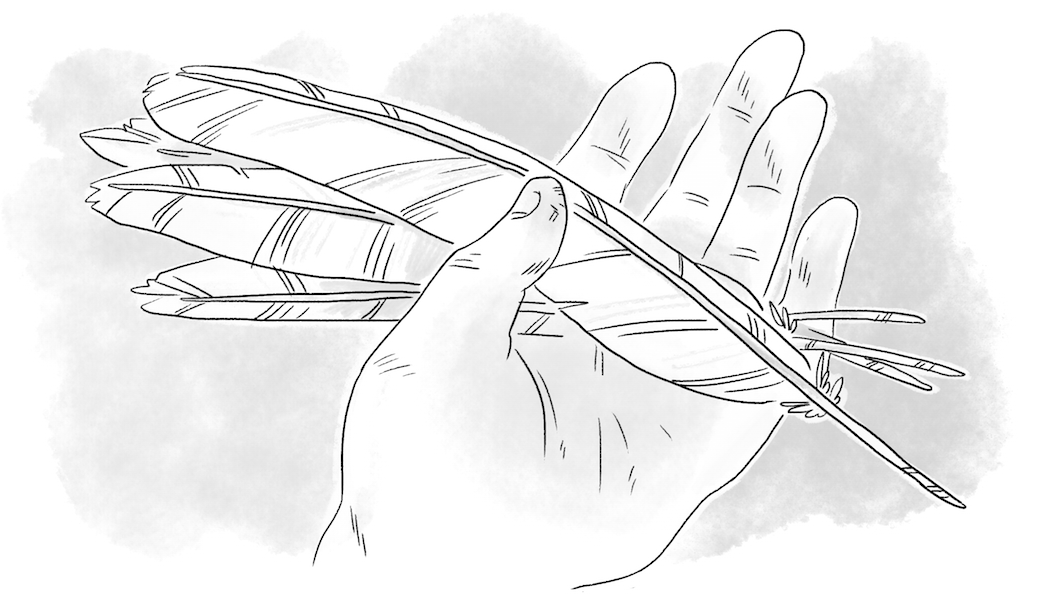
\includegraphics{img/hand_and_feathers.png}
  \caption{}
  \end{figure}
  
  The hole led to a narrow passageway that ran along the edge of the
  cliffs. The rock had been carved away to make a tunnel just big enough
  to walk through with your back bent low. Dirt and sand covered the
  floor. Captain Z could see a light coming from the doorway at the far
  end.
  
  As she walked through the tunnel, she thought she heard a voice above
  her. Someone shouting. Captain Spears was close. Somehow he and his crew
  had found the path up the cliffs. But the voice was faint, its owner
  still far away. Captain Z kept going. Crouching, she walked to the end
  of the passage, and into a little cave.
  
  The cave was bright. Another hole along the side of the far wall acted
  like a window. The window opened up to the cliff side, and the sun and
  sounds of the waves below and the gulls above were coming in.
  
  Captain Z looked around.
  
  There in the corner of the cave nearest the door was a pile of rocks.
  Captain Z stepped over to it and quickly but carefully started pulling
  the rocks off the pile.
  
  Six or seven rocks down, she saw it. A little leather bag.
  
  Now treasure is is often kept in a chest. Sometimes, gold is found in
  big sacks. Sometimes, necklaces and rings can be found in a jewelry box.
  Captain Z had never heard of a treasure found in a little leather bag.
  
  Still, she reached for it just the same. \emph{Perhaps its a message
  telling where the real treasure is hidden,} she thought. She tried to
  ignore the idea that someone before her had already grabbed the
  treasure, and this was just what they had left behind.
  
  The bag felt empty. And when she opened it at first she didn't see
  anything. Her heart sank. But then she stuck her hand in, rummaged
  around, and pulled out four feathers and a scrap of paper.
  
  She looked over the feathers. They were bright white, but otherwise
  quite ordinary. About the size of crow feathers, perhaps just a bit
  bigger. She didn't recognize the bird they had come from, but they
  didn't seem particularly interesting.
  
  She looked at the paper. There were words on it that looked to be a
  poem.
  
  \emph{Only one of true measure,}
  
  \emph{can make use of this treasure.}
  
  \emph{But on a person or steed worn,}
  
  \emph{these feathers make a hero born.}
  
  \emph{Not from a bird or bat of course,}
  
  \emph{but from the only winged horse.}
  
  \emph{The gods were surely right to bless,}
  
  \emph{the feathers of the Pegasus.}
  
  Feathers?
  
  Feathers were the treasure of Castle Island? Captain Z's heart sank.
  Certainly this was some trick. Some terribly unfunny joke.
  
  The sounds of laughing and talking in the tunnel outside the cave made
  the hair on the back of her neck stand up.
  
  \emph{A joke that isn't very funny,} she thought as she looked for a
  place to hide.
  
  She didn't have more time to curse the feathers or even think about them
  anymore.
  
  Captain Spears and his crew had found her.
  
  \section{}\label{section-20}
  
  Haphazardly and out of habit, Captain Z shoved the feathers into one of
  the many pockets on her vest.
  
  It turns out that this thoughtless action was in fact a very good
  thought indeed, as we shall find out.
  
  The pirates came into the cave. Smiling cruel smiles and waving their
  cutlasses about. With the leather bag in her hands, Captain Z backed up
  further and further till she was right in front of the little opening in
  the cave wall that looked out to the sea.
  
  If she stayed in the cave, the treasure would be lost, and maybe worse.
  She decided to try her luck out of the cave. Perhaps there was a way
  down.
  
  She turned to the little window and before any of the other pirates
  could grab her she was out on a ledge outside the cave. The wind was
  blowing hard and there were just a few spots in the rocks to hold on to.
  
  Captain Z looked down to see the ocean crashing into the rocks below.
  Those rocks looked big and sharp, even from up there. One slip, and she
  was a goner. Perhaps this wasn't such a good idea, she thought to
  herself.
  
  She tried to shimmy away from the window to the cave, but didn't get
  far. The ledge stopped short a little ways past the hole. There didn't
  seem like there was any other place to put her feet. She was stuck.
  
  Captain Spears and Hissy ducked into the cave last after his crew. He
  saw Captain Zephyr's legs as she went through the hole.
  
  His eyes went from cool confidence to wild panic, all in one second.
  
  \enquote{She's escaping you fools! Grab her!} He shouted. The pirates
  closest to the hole looked out, but didn't move. They weren't eager
  about following Captain Z out the window. They just stood where they
  were, looking back and forth between the frightful Captain Spears and
  the terrifying cliff wall.
  
  Captain Spears pushed past them. \enquote{Ya good-for-nothings,} he
  muttered.
  
  He himself pushed his head and shoulders through the hole to look out on
  to the other side.
  
  \section{}\label{section-21}
  
  There was Sophia Zephyr, stuck on the edge of the ledge, just out of
  reach. She was holding on to a little leather bag and trying to find a
  way down the cliff side, without much luck.
  
  Captain Spears considered going out on the ledge himself to get the
  treasure bag. Then he looked down at the rocks below and thought better
  of the idea. Maybe he could talk her back inside.
  
  \enquote{Tis over, Zephyr,} he said with a smirk. \enquote{Give me the
  bag, and we'll get you back to solid ground.}
  
  \enquote{Walking the plank doesn't seem so solid to me,} Captain Z shot
  back. Her arms were aching. She wouldn't be able to hold on much longer.
  
  \enquote{On my mother's own watery grave,} said Spears, trying hard to
  look honest, \enquote{not a hair on your pretty head need be harmed if
  you give up the booty now.} Then he looked down with a grin.
  \enquote{Unlikely, I'd say, you'd get such a promise from those rocks
  down there.}
  
  Captain Z didn't trust Spears one bit, but what other choice did she
  have? The game was up.
  
  Slowly, Captain Z shuffled back toward the window to the cave.
  
  Captain Spears stepped back and watched as she got closer, so as not to
  scare her. They would deal with her once the treasure was out of her
  hands and into his.
  
  From outside the window, Captain Z tossed the treasure bag that had
  caused all the trouble in to the cave. The pirates all jumped on the
  bag, pushing and pulling, each one wanting to be the first to see the
  treasure first. Not one of those scoundrels suspected the treasure,
  useless as it looked, happened not to be in the bag.
  
  But Hissy knew something wasn't right. As Captain Zephyr reached for the
  window to pull herself in, that meanest of cats ran up to her with a
  growl. It bit into Captain Z's vest pocket, pulling out one of the
  feathers she had hidden there.
  
  Captain Z grabbed for the feather, snatching it out of Hissy's mouth.
  But as she did, her other hand slipped from the rock.
  
  She didn't even have time to scream as she fell backwards, down to the
  rocks and the sea below.
  
  \section{}\label{section-22}
  
  \begin{figure}[htbp]
  \centering
  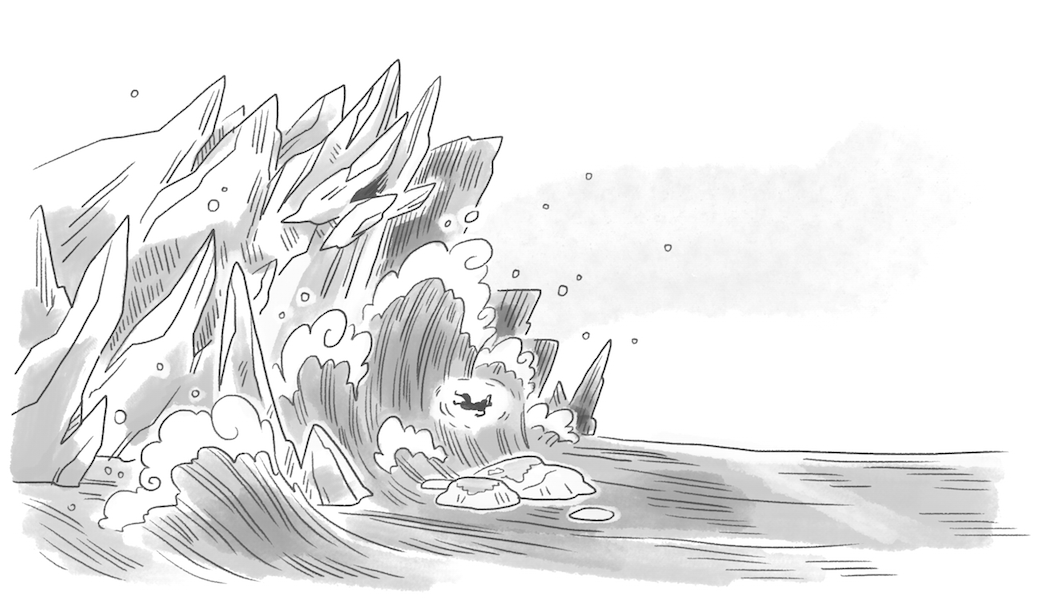
\includegraphics{img/fall_from_castle_island.png}
  \caption{}
  \end{figure}
  
  The captain's eyes were shut tight while she braced for the crash. She
  expected the end to be terrible.
  
  But the end never came.
  
  After what seemed like forever, Captain Z bravely opened one eye, just a
  peak. Then she opened it a bit wider. Then both eyes. Then both eyes
  wide.
  
  She wasn't falling down. She was floating down!
  
  She drifted down the cliff side, the way a dandelion seed might dance on
  the breeze.
  
  By the time she made it to the crashing waves and the rocks, her legs
  were beneath her. She touched down gently, her feet resting on the top
  of a mossy rock.
  
  Looking all around for an explanation, she saw none. She looked up at
  the hole from which she fell. It looked tiny from down here. She looked
  around at the ocean and the waves crashing around her. Then she looked
  at the feather in her hand.
  
  A feather?
  
  She stared at it, unbelieving. She put it in her pocket. Immediately
  when she took her hand out, all her weight came back. Her body felt
  heavy and her legs felt weak. She stumbled onto another rock and reached
  out to balance.
  
  She looked up again to see if anyone was watching from the hole in the
  cliff. No pirate heads were sticking out to see her fall. Above the
  cliffs the gulls continued their calls and cries. Out of that mess of
  birds swooped Muddle. She coasted on the breezes above Captain Z's head.
  They were glad to see each other.
  
  Captain Z picked her way among the rocks, making her way as fast as she
  could back toward the beach where her boat was hopefully still docked.
  
  \emph{Those pirates up in the cave will no doubt be angry when they find
  that leather bag empty}, she thought. If they thought her gone, then all
  the better. That way, they wouldn't be chasing her now to reclaim the
  treasure.
  
  \section{}\label{section-23}
  
  Up in the little cave on the side of the cliff, the pirates were still
  fighting over who would open the satchel of treasure.
  
  In fact, it was such a fight that no one but Hissy and Barnacle Bill had
  noticed Captain Z's fall.
  
  Bill had stayed out of the fight over the bag, as he didn't want to get
  hurt in the scuffle. He was on the other side of the cave, near the
  doorway when he saw Hissy try for the feather and watched in horror as
  Captain Z slipped and disappeared from view. In fact, it was such a
  terrible sight that he just stood there with his mouth open wide and his
  eyes opened wider, as the others continued to fight.
  
  Golden George had grabbed the bag away from Smelly Ned, who had pushed
  poor old Jon Thumb down to get it. But now they were all wrestling on
  the floor again.
  
  \enquote{Enough ya sea rats,} their captain bellowed. \enquote{Hand me
  the booty.}
  
  That was the end of the fight. Golden George reluctantly held out the
  bag for Captain Spears to take.
  
  \enquote{Well it ain't foods,} said old Jon Thumb, with a hint of
  sadness. He and Cinnamon the cook had spun tales of the meals they would
  eat here on the island.
  
  \enquote{Is it gold?} Asked Golden George.
  
  \enquote{Nay,} said Spears with a frown. \enquote{Not heavy enough a
  sack,} he said, raising the bag up and down.
  
  \enquote{Looks small,} said Sally Snake Eye.
  
  \emph{it does,} thought Captain Spears. The thought that they had been
  bamboozled crept into the back of his mind. Quickly, he opened the bag
  and looked in with his good eye.
  
  He stood there peering into the bag for a full minute. He didn't believe
  what he saw.
  
  \enquote{Well, captain,} Sally Snake Eye finally spoke up.
  \enquote{What's in the bag?}
  
  Captain Spears turned the bag upside down. Only a bit of dust fell out
  and floated to the ground.
  
  All eyes turned to the little hole that Captain Z had gone through. Now
  it dawned on them that she hadn't come back through it.
  
  Spears ran to the hole and stuck his head through. He looked back and
  forth along the cliffs and saw nothing but stone.
  
  He pulled his head back in and looked around at his crew.
  
  \enquote{Where did she off to?} he said in a low voice. Not really a
  question to the crew, but this was the cue for Barnacle Bill to finally
  speak up.
  
  \enquote{H-H-Hissy!} He stammered.
  
  \enquote{Hissy what?} Spears said, glancing at the cat. She was near the
  window cleaning her paws, as if nothing at all had happened.
  
  \enquote{Hissy pushed her out!} Bill responded. His wide eyes locked
  onto the cat as he pointed. \enquote{Down down down,} he said sadly and
  trailed off.
  
  Captain Spears pushed his head through the hole again and looked down to
  the crashing waves below. He peered with his red eye hoping to see some
  sign of Zephyr in the ocean froth. Much as he hoped, he saw nothing.
  
  He pulled back and swatted at the mean cat with his hat. She ran a few
  feet, hissing, then stopped again to clean another paw. Spears turned
  back to his crew with his eyes down to the ground.
  
  \enquote{Escaped?} Asked Smelly Ned. Perhaps she had caught another part
  of the cliff.
  
  Captain Spears shook his head no.
  
  \enquote{I fear she took the long fall,} he said.
  
  Even though she had stolen the map and the treasure from them, the whole
  crew was more sad then mad as they walked slowly down the trail.
  
  It's a sad thing to loose a pirate.
  
  They had looked through the rest of the rock pile and all through the
  cave for where the treasure might be hiding. Nothing but more dust was
  found.
  
  They would search the rocks below the cliffs for the treasure for the
  rest of the day. But, of course, they would find nothing.
  
  Meanwhile Captain Z was on her way to getting off the empty bit of land
  known as Castle Island.
  
  \section{}\label{section-24}
  
  Captain Z had been rowing for an hour and was getting close to a tiny
  cove behind a jagged little mountain, on the south end of the island.
  This was the place she had hidden her boat, Wind Drinker.
  
  Captain Spears and his crew hadn't seen the spot, as they came down from
  the North and had stayed anchored in plain sight. They weren't looking
  for a place to hide, as they didn't expect to find anyone here.
  
  But Captain Z had done things differently. When she had sailed for
  Castle Island, she had come around wide during the night. The little
  cove was a lucky find, and the perfect spot for her boat. That giant
  monster of a boat, Captain Spears's Sea Breaker, probably wouldn't have
  fit anyway.
  
  Wind Drinker was different. Captain Z was the entire captain and crew of
  the whole ship. It was tricky, but with her custom riggings, cranks, and
  cables, the boat could be managed by a crew of one. Captain Z had made
  it all the way to Castle Island by herself.
  
  Captain Z rowed around the bend at the southern tail of the island and
  slipped into the little cove. Wind Drinker was there waiting for her.
  Muddle cawed from above and landed on the ship's front mast.
  
  \begin{figure}[htbp]
  \centering
  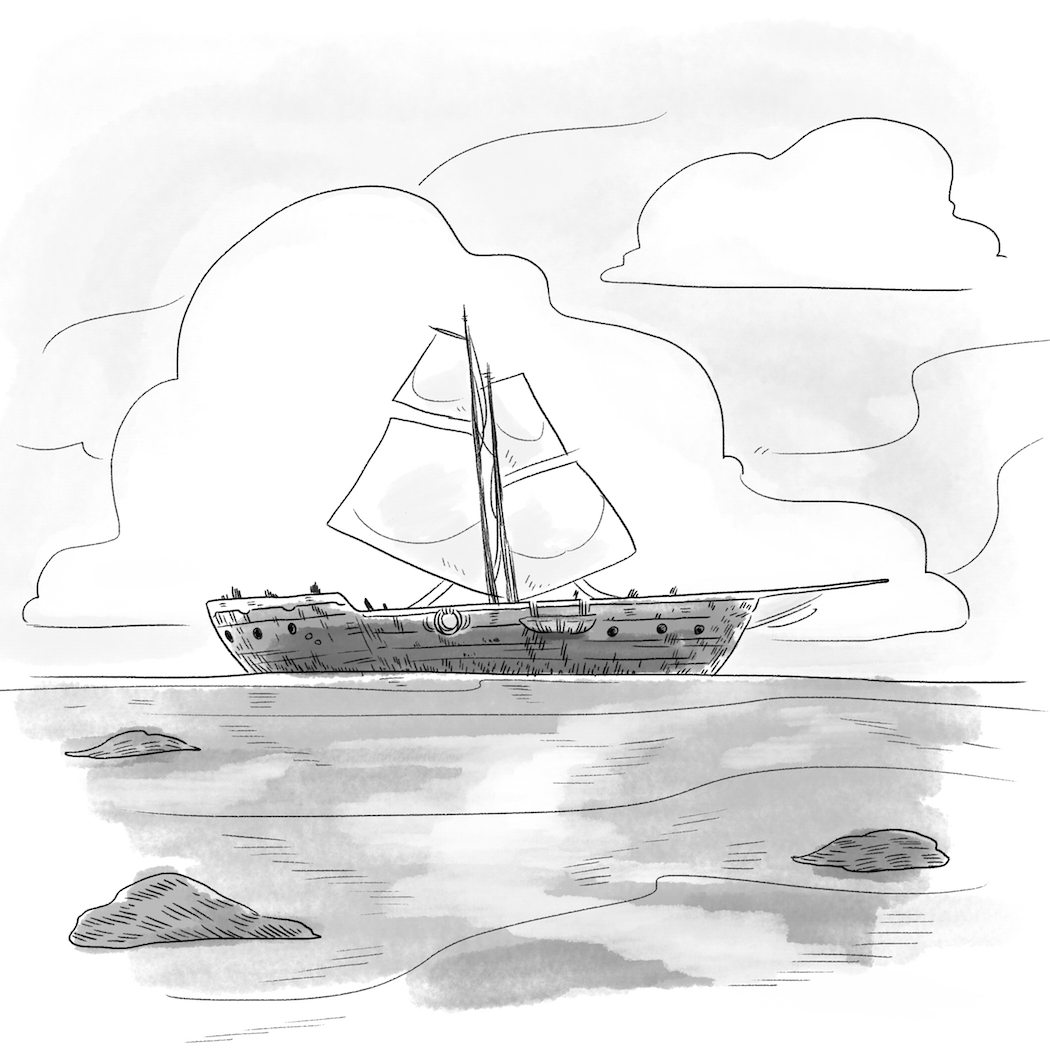
\includegraphics{img/wind_drinker.png}
  \caption{}
  \end{figure}
  
  There was a ladder and a hook attached to a rope on the back end of the
  ship. Captain Z fixed the hook on the front of the rowboat, then used
  the ladder to get on deck.
  
  She turned a crank that pulled in the rope and hoisted the rowboat up
  out of the water and on to the back of the ship. It was a tight spot,
  but she knew it would all fit as it had before.
  
  Cranks clanked and spinners spun as Captain Z prepared to launch. All
  the sails of Wind Drinker were raised by the cunning pirate. The anchor
  was pulled and then, before you could say \enquote{Jolly Roger}, the
  ship had set sail.
  
  Captain Z was still confused, and a bit sour, about the treasure.
  Feathers weren't on the top of her list of valuable booty. She wanted
  gold. She wanted jewels. She wanted a diamond the size of her fist!
  
  Still, floating down that cliff and making it to the bottom without a
  scratch, must be worth something. She pulled out the poem and read it
  again, trying to figure out what it meant, but only getting more
  confused.
  
  She had heard the name Pegasus, but didn't remember from where. And she
  didn't understand how these feathers might help make heroes.
  
  Also, in her hand was the jumbled letter from Captain Spears's chest.
  This thing was valuable to Spears, else he wouldn't have locked it up.
  Perhaps it was worth something to her as well.
  
  She wanted a second set of eyes to read these words, to see if more
  information could be squeezed out of them. And she knew just the person
  who was best at squeezing out information.
  
  Captain Z set course for the Port of Goodnews, the biggest town in the
  West Waters, and the home of her good friend, Dr.~Nora Star.
  
  \section{}\label{section-25}
  
  The fast sails of Wind Drinker brought Captain Z to the Port of Goodnews
  as night fell on the city.
  
  The harbor master was paid extra to keep his mouth shut about the ship,
  but Captain Z knew it hardly mattered. If someone wanted to find out she
  was there, it would happen. She would be gone soon anyways. Since she
  had turned to pirating, Goodnews wasn't the kind of town she liked to
  stay in long.
  
  She walked through the crowded streets, winding around familiar
  restaurants and stores until she made it to the quiet little alley known
  as Incident Avenue. Two blocks down and there was Dr.~Star's home and
  workplace. The sign above it read \emph{Star Light, Star Bright:
  Schooling and Support for Children in Need}.
  
  It was well past closing time, but Captain Z knocked just the same.
  After a few minutes, she could hear someone behind it walking up.
  
  \enquote{We're closed,} a voice shouted. Captain Z could tell it was
  Nora, trying to sound sterner then she was.
  
  \enquote{Well, then you better open back up,} Captain Z responded.
  
  \enquote{Sofia, is that you?} Nora opened the door a crack to look
  through. Then she opened it all the way and ran out to give her friend a
  hug. It had been nearly a year since they had last seen each other.
  
  \enquote{I have some questions for you,} Sofia Zephyr said, looking a
  bit sorry that she hadn't come just to visit.
  
  \enquote{I figured as much. Let's get inside,} said Dr.~Star.
  
  The two walked into the boarding school and closed the door behind them.
  
  \section{}\label{section-26}
  
  Sophia Zephyr still knew her way around all the odd twists and turns to
  get to the main room. Although it had been a year since she last
  visited, it was still all very familiar. As a child, Sophia had grown up
  inside this school.
  
  Orion and Nova were both reading by lamp light. When they saw Captain Z
  in the doorway they both sprang up to give her a hug.
  
  Little Lucy had fallen asleep on the floor. With all the commotion she
  woke up, but stayed on the rug rubbing her eyes. She was five now, but
  had joined the school a year ago after being rescued by Dr.~Star.
  
  Because she was so young when Captain Z had visited last, Lucy didn't
  recognize her, and she didn't trust anyone she didn't recognize.
  
  Nova and Orion wanted to hear stories of Captain Z's latest pirate
  adventures. So she told them of her run-ins with Captain Spears and the
  hunt for treasure on Castle Island. She skipped over talking about the
  feathers and the falling from the cliffs for now. She wanted to talk to
  Dr.~Star about that first.
  
  Soon, Lucy was in Captain Z's lap listening with rapt attention. Just
  like that, Sophia and Lucy became fast friends again. Like Sophia, Lucy
  had a bit of a wild streak and a love for excitement and danger.
  
  As Sophia finished talking, Lucy was so tired that she was carried off
  to bed by Dr.~Star. Captain Z got a few more hugs from the other two
  children. Then, Nova put her arm around her younger brother Orion and
  the two walked back to their room to collapse into their soft beds under
  warm blankets.
  
  But the night was still early for Dr.~Star and Captain Z.
  
  \enquote{I've got something I want to talk to you about,} Sophia said to
  her old mentor.
  
  \enquote{I'm all ears,} Dr.~Star responded.
  
  \section{}\label{section-27}
  
  Captain Z showed the feathers to Dr.~Star and read her the poem.
  
  \emph{Only one of true measure,}
  
  \emph{can make use of this treasure.}
  
  \emph{But on a person or steed worn,}
  
  \emph{these feathers make a hero born.}
  
  \emph{Not from a bird or bat of course,}
  
  \emph{but from the only winged horse.}
  
  \emph{The gods were surely right to bless,}
  
  \emph{the feathers of the Pegasus.}
  
  \enquote{So what does it mean?} She asked the doctor after she had
  finished. \enquote{What is a \emph{Pegasus}?}
  
  \enquote{Well, the Pegasus is a myth. A legend,} Dr.~Star explained.
  \enquote{The story goes that there once was a terrible monster, Medusa.
  She had snakes instead of hair and was so frightening that anyone who
  looked at her was turned to stone.}
  
  \enquote{Sounds like a nice lady, wish I could have met her,} Captain Z
  joked.
  
  Dr.~Star continued. \enquote{Eventually, a hero comes and kills her.
  Cuts her head clean off. But out of Medusa's body springs the winged
  horse Pegasus. This Pegasus is the fastest horse in the world, with the
  added benefit of being able to fly. The Pegasus is in all sorts of
  stories where it helps heroes battle monsters, or fly to the gods, or
  other such fun.}
  
  \enquote{Do any of these stories have pirates in them?} Captain Z asked.
  
  Dr.~Star laughed. \enquote{Not that I remember,} she said.
  
  \enquote{Well how can it be that I have the feathers of a mythical
  flying horse?}
  
  \enquote{I don't know,} Dr.~Star responded. \enquote{It sounds like a
  hoax.}
  
  \enquote{But that's the crazy part. They worked for me,} Captain Z
  retorted.
  
  \enquote{What do you mean by that?} Dr.~Star was confused.
  
  Sophia filled in the parts of the story of Castle Island that she had
  left out the first time she told it. How that mean cat Hissy caused her
  to fall. How instead of smashing onto the rocks, she had held on to the
  feather and floated down.
  
  Dr.~Star frowned. \enquote{That's unbelievable.}
  
  \enquote{You're right,} Captain Z said as she smiled. \enquote{I don't
  believe it myself. But that doesn't mean it didn't happen.}
  
  \enquote{But if the poem is right,} she continued, \enquote{then only a
  hero would be able to fly with these things.}
  
  \enquote{Well then, maybe you aren't really a pirate,} Dr.~Star smiled.
  \enquote{Perhaps there is a bit of hero in you after all.}
  
  Now Captain Z frowned. She had never heard of a hero pirate. Those words
  didn't make much sense together in her ears.
  
  \enquote{One last question about this then,} Captain Z said.
  \enquote{Does steed just mean horse? If I had a little pony to ride, it
  would be floating too?}
  
  Dr.~Star thought for a bit. \enquote{That's what the word steed usually
  means,} she said finally. \enquote{But it could be that the poem is
  saying it that way just to rhyme. Perhaps anything ridden could count as
  a steed. I can't say for sure.}
  
  \emph{If that were true,} she thought, \emph{my steed would be Wind
  Drinker.} That was an exciting thought. A flying ship would be a whole
  lot more useful then a flying horse to a pirate.
  
  \section{}\label{section-28}
  
  Both women were very tired, it had been a long day. Dr.~Star yawned and
  started to get out of her chair to go to bed.
  
  \enquote{Let's get some shuteye} Dr.~Star sighed. \enquote{We can tour
  the town tomorrow. See all the friendly faces.}
  
  \enquote{Probably not many of them left,} Captain Z grumbled. Then she
  pulled out an envelope from her vest.
  
  \enquote{Just one more thing,} she said. It was that paper with the
  jumbled letters on it she had found with the map. \enquote{What do you
  make of this?} She asked the doctor.
  
  Nova looked it up and down for a long time, holding it close to the lamp
  to see better.
  
  \enquote{This looks like a code to me,} she answered finally. \enquote{A
  hidden message of some sort. I've heard of a way to hide a message that
  would look like this. First you switch all the letters around. A becomes
  P, B becomes T, and so on. Then you write your message with this new
  alphabet arrangement.}
  
  Dr.~Star paused a moment to yawn. Then she continued.
  
  \enquote{Anyone who needs to read the real words knows which way the
  letters were swapped, so its easy for them. To everybody else, the
  letters don't make sense.}
  
  \enquote{Could \emph{you} make sense of it?} Asked Captain Z hopefully.
  If Dr.~Star could crack the code, then maybe it would lead to more
  treasure.
  
  \enquote{I've never been any good with words and puzzles like this,}
  Dr.~Star said shaking her head. \enquote{It would take me weeks, and I
  might not get anywhere.}
  
  Captain Z took the paper back and looked at it a bit longer.
  
  She was pretty good with words, when she wanted to be. Maybe she had
  enough smarts to crack the code. But it would have to wait for a time
  when she wasn't so tired.
  
  The night ended with a hug. Captain Z found a cozy couch and a warm
  blanket and was soon deep asleep. Snoring, and dreaming of hidden
  treasures to be found.
  
  \section{}\label{section-29}
  
  The next morning, bright and early, Sophia was woken up by the banging
  of pots and pans in the kitchen. When she staggered in to see what was
  making all the commotion, she found Lucy. Lucy had decided she wanted to
  make everyone breakfast, and was trying her best to figure out how.
  
  Captain Z offered to help.
  
  By the time the rest of the group was awake, they had coffee, eggs,
  pancakes, and fresh strawberries on the table. Everyone thanked Lucy and
  Sophia, for the delicious start to the day.
  
  After they had cleaned up, it was time for Dr.~Star to get to work. She
  had some patients to see and didn't want to keep them waiting.
  
  \begin{figure}[htbp]
  \centering
  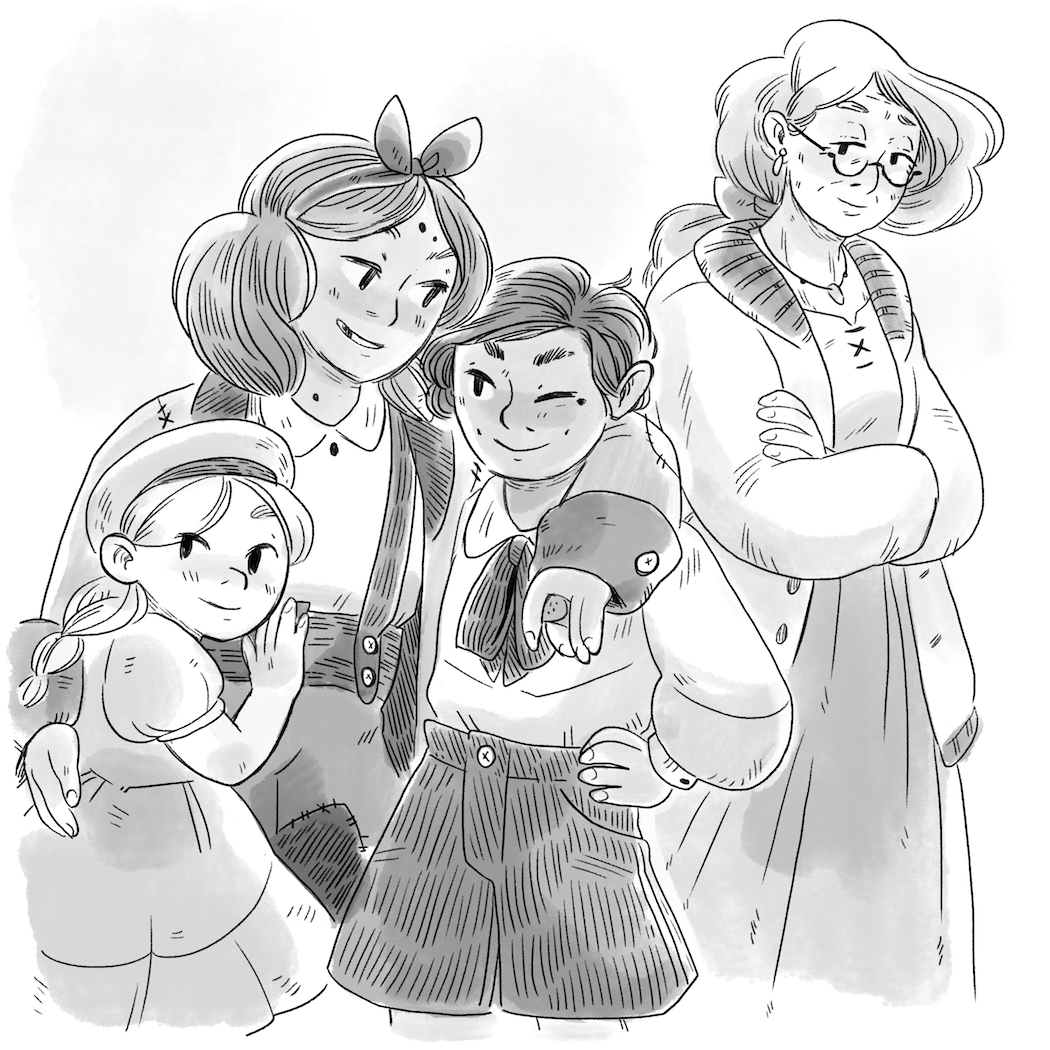
\includegraphics{img/dr_star_n_kids.png}
  \caption{}
  \end{figure}
  
  \enquote{Why don't you all go into town together,} she said as she was
  packing up her things. \enquote{You can go see Walter and get some food
  at the market for supper tonight.}
  
  While Captain Z wasn't too excited about taking three children around by
  herself, it would be nice to see her old classmate. She hadn't seen
  Walter since her last visit when he helped her with the special riggings
  and cranks on Wind Drinker.
  
  It was a short walk down the hill and into the market. The streets were
  already crowded that morning. It seemed like everyone in town had come
  out to buy fish, fruit, or trinkets. Captain Z pushed her way through
  the crowds, making sure that the children stayed close behind.
  
  Eventually, they reached the quieter end of the market and ducked into a
  dark and smoky little building. Inside was Walter, the blacksmith. He
  was banging away on a piece of red hot metal, sweating and scowling at
  it as he shaped it into a point. It looked to be some new type of spear,
  most likely made for the town guard, they were his best customers.
  
  Sophia had grown up with Walter in Dr.~Star's school. They had both been
  part of the very first class when Dr.~Star first opened the school.
  There were two boys and two girls in that class, and Walter and Sophia
  were one of each. They had been like brother and sister back then,
  always joking around, but also always watching out for one another. Even
  now that they were both grown up, they still acted a bit like siblings
  when they got together.
  
  Walter didn't even have to look up to know who had come into his shop.
  He could tell it was Sophia just by her walk.
  
  \enquote{Well, did you get another boat you need to rig with pulleys?}
  Walter asked. He looked up and smiled at Captain Z.
  
  \enquote{I'm still enjoying the first one too much to be needing
  another,} Captain Z responded.
  
  Walter put down his fired metal and gave Sophia a big bear of a hug. He
  was stronger than he looked, all that blacksmithing builds muscle.
  
  The children walked around the little shop to admire Walter's creations
  as the two grownups talked. Walter liked making little figures when he
  wasn't working on weapons. On his shelves stood a little metal knight,
  complete with sword and shield, and a wonderfully detailed little metal
  dragon. It looked as if it might come alive any second to fly about the
  room.
  
  \enquote{It's good to see you, Little Z,} Walter said. That was the name
  he had given Sophia while they were in school together. She had always
  been shorter and smaller then the others. Captain Z was now taller then
  Walter by a few inches, but the name stuck.
  
  \enquote{It's good to see you too Walter,} Captain Z said.
  \enquote{What's new in Goodnews?}
  
  \enquote{Ah, everything stays the same 'cept what's been changing,}
  Walter said with a wink. He never had a straight answer to a question.
  
  Captain Z asked about the others they had gone to school with when they
  were young. Besides Sophia and Walter there were Irene and Carlos. Irene
  was still at the university, her head filled with enough facts and
  understandings for ten people.
  
  Carlos was still missing. No one had heard from him in three years.
  Walter feared the worst.
  
  \enquote{Can't be nothing but trouble for Carlos, says I,} Walter
  remarked.
  
  \enquote{I'm sure he will come back someday,} Captain Z said.
  
  Walter grunted. He didn't think she was right about that, but there was
  no reason to argue the point.
  
  \enquote{One thing that has changed around here is the guards,} Walter
  said, peering out the door before continuing. \enquote{Lately every one
  of them seems to be getting up on the wrong side of the bed. The
  prison's overflowing with all the people they've locked up. It would
  seem just looking at them wrong is enough reason for them to drag you
  away these days.}
  
  \enquote{Any ideas as to what's keeping them in such mean spirits?}
  Captain Z asked.
  
  \enquote{I'm not one for ideas,} Walter said. \enquote{Those I have I
  keep to myself, especially since they are still eager to buy my wares.
  Irene might be having an opinion on the matter. You should go ask her.}
  
  Walter and Captain Z talked for a bit longer, retelling stories from
  their childhood. Then it was time for Walter to get back to his
  metalwork. They hugged again and said their goodbyes. Captain Z promised
  to come back for a longer chat in a few days. Then she and the children
  went on their way.
  
  \section{}\label{section-30}
  
  They walked back out on to the street and down towards the market.
  
  \enquote{I'm hungry,} Nova complained.
  
  \enquote{Let's get some lunch at one of the market stalls,} Captain Z
  suggested. \enquote{Then I'll take you into the University before we
  head home.}
  
  Irene, the other girl in Dr.~Star's first class would mostly likely be
  among the books and papers there. Perhaps she could help crack the note
  Sophia had found on Captain Spears's boat. Irene had helped design the
  pulleys and mechanisms that Walter had made to allow Captain Z to sail
  Wind Drinker solo. She seemed to know something about everything.
  Uncovering the hidden message might make for an easy task for her.
  
  They walked through the market stalls looking at all the food and wares
  for sale. Exotic spices filled one stall, their scents spilling out into
  the street and into their noses. Fresh fish were in another, some bigger
  than a man hung from the rafters. A few sellers had huge wheels of
  cheese on their tables and sausages linked together in long chains. Some
  stalls had silks and scarves and brightly colored cloth for sale.
  
  The crowds were filled with all sort of folks who were out enjoying the
  sights, smells, and tastes of the market. Families were strolling
  through to buy groceries for dinner. Merchants were perusing the stalls
  hoping to find good deals on silks or spices that they could resell in
  the smaller towns on the nearby islands. Town guards were roaming about
  in packs of two or three. There seemed to be a lot of them, and most
  seemed to have a sour look on their faces, from what Captain Z could
  see.
  
  \emph{A bit unusual for such a nice day as this,} she thought.
  \emph{Most likely its all in my head, I'm seeing things because of
  Walter's words. But than Walter is always suspicious about something or
  somebody.}
  
  As they walked, the bright colors of fresh fruit caught Lucy's eye and
  she went over to a large stand to admire them. The stand had dates and
  plums on their tables, along with baskets of lemons and oranges. Limes
  were in great big barrels, alongside large juicy looking apples.
  
  Lucy reached into one of the barrels and pulled out the biggest apple
  she had ever seen. She could barely hold it in one of her hands. She
  held it up and looked at it. Fruit like that rarely made it to the Port
  of Goodnews. Most of it was sent directly to the big cities of the
  Eastern Coast, where prices were higher and tastes were fancier.
  
  \enquote{Look!} She said to the others.
  
  Captain Z saw Lucy holding the apple and smiled. But her smile faded
  when she saw two guards came up behind Lucy with anger in their eyes.
  
  \section{}\label{section-31}
  
  One of the guards grabbed Lucy's wrist. The apple dropped down to the
  ground, rolling under the fruit seller's market stand.
  
  \enquote{Gotcha!} The guard shouted. \enquote{Thought you'd be running
  off with a nice red apple, did you? Well think again! You're coming with
  us. Thieves like you get locked away in Goodnews.}
  
  Captain Z ran up to the guards. Lucy twisted her wrist free and jumped
  behind Captain Z as she stopped in front of them.
  
  \enquote{What are you doing?} She asked. \enquote{The girl's done
  nothing wrong, she's with me. Where are you trying to take her?}
  
  The second guard snorted. \enquote{That street urchin was fixing to
  steal fruit from one of our honest sellers here,} he said. \enquote{It's
  a good thing we were here to stop her, isn't that right?}
  
  The guard was looking at the fruit seller for a reply. The old man had a
  big belly and a balding head. Behind his glasses, his eyes shifted back
  and forth between Lucy, Captain Z, and the guards.
  
  \enquote{Listen now,} he stammered. \enquote{I don't want any trouble.}
  
  \enquote{This thief is the one in trouble here not you,} the first guard
  said with a mean looking smile. \enquote{She was trying to take that
  apple from you, right?}
  
  The old man's eyes flicked back and forth even faster. His breaths were
  short and close together. \enquote{Well, well, well\ldots{} I wasn't
  paying much attention,} he said finally. \enquote{But, if you say so.
  I'll trust your word officers.}
  
  Captain Z interrupted before the guards could respond.
  
  \enquote{In any case, it's not stealing if you get paid. Here's the two
  coppers for that apple, and one more for your troubles.} She plunked
  three coins down on the table and turned around. She grabbed Lucy's hand
  and started to walk back to the other children who were standing in the
  road looking worried.
  
  \enquote{Say now!} Called out one of the guards. \enquote{Don't you want
  your apple?}
  
  Captain Z turned around. One of the guards were moving slowly around the
  stand towards her and the children. She had a hunch that they weren't
  going to let them get away easily. The other picked up a mushy looking
  apple off the ground, not the one Lucy had picked, one that had been
  rotting there for some time.
  
  \enquote{That money bag of yours looks full of silvers. Maybe even a bit
  of gold,} he said. \enquote{One little apple must not mean much to you.}
  
  He tossed the apple to Captain Z who caught it with one hand.
  
  \enquote{Ya, pirate,} he finished.
  
  \section{}\label{section-32}
  
  Hearing that word made all other people around them in the market stop
  and stare at the captain. As Captain Z knew, pirates were forbidden to
  enter Port Goodnews. Any pirate caught in town could be locked up for a
  very long time.
  
  Even if you weren't really a pirate, just being called one could get you
  into a lot of trouble. Captain Z had learned these lessons the hard way.
  
  \emph{He would have branded me a pirate no matter what I did,} Captain Z
  realized. \emph{But unlucky for them, it happens to be true.}
  
  The guards inched closer.
  
  Captain Z felt the apple in her hand. She threw it hard underhanded
  straight from her hip. It caught the nearest guard square in the
  forehead, hitting him hard with a thump. He nearly fell over from the
  blow and stood there holding his head, apple mush all over his face.
  
  Captain Z took off.
  
  Grabbing Lucy's hand again, she started running away from the fruit
  stand.
  
  \enquote{Let's go!} She ordered the other two children. Nova and Orion
  followed, running as fast as they could.
  
  People in the crowd watching the ordeal jumped back as the guards pulled
  out their swords and started following. The first guard was still wiping
  the mush off as he ran.
  
  \begin{figure}[htbp]
  \centering
  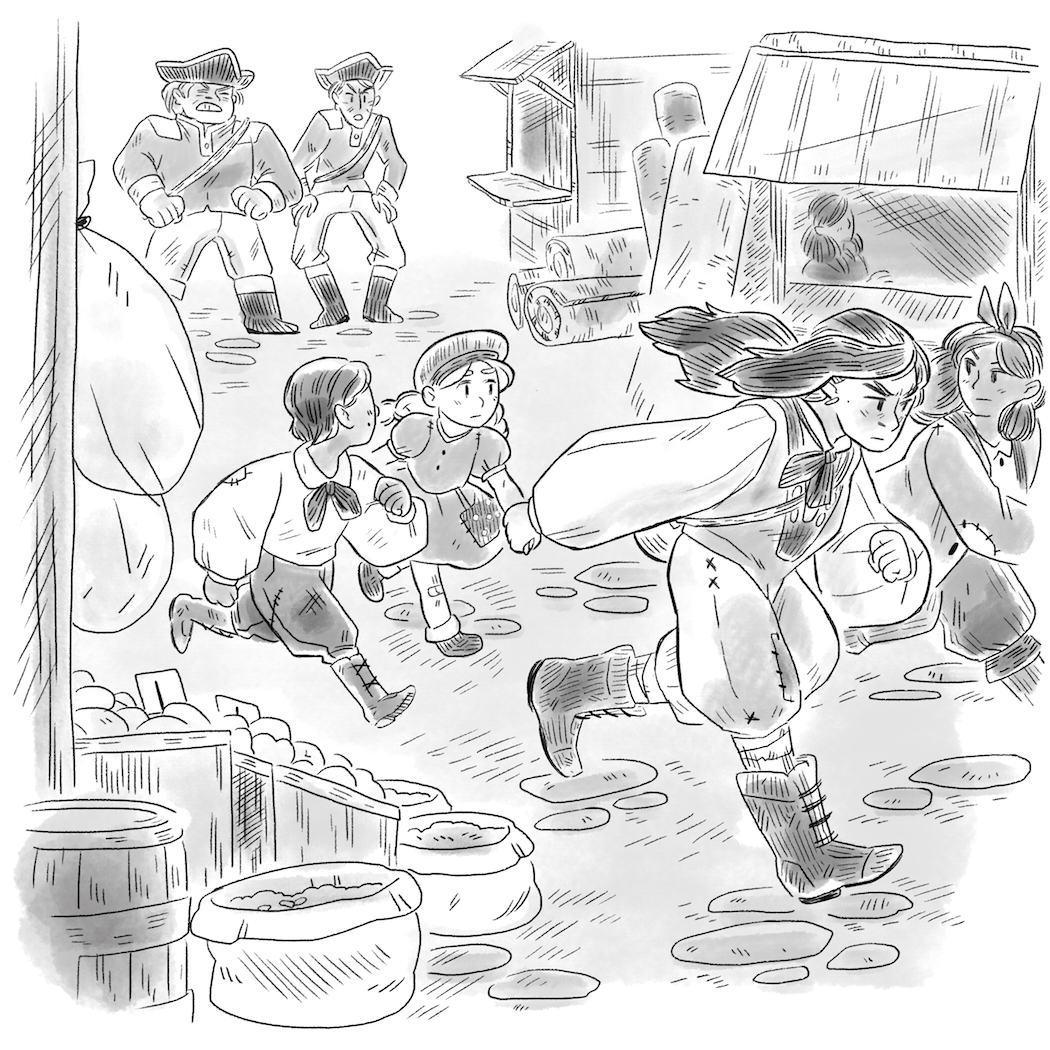
\includegraphics{img/running.png}
  \caption{}
  \end{figure}
  
  The apple had slowed the guards a bit, but not by much. Captain Z tried
  to loose them in the crowds by running zip-zag through the stalls and
  people. Still the guards followed. They were getting closer.
  
  Captain Z led the children out of the market and into a little alleyway
  between the nearby stores. They ducked under low hanging wires crowded
  with drying clothes. They sped left, then right, down through a maze of
  side streets, trying to loose the guards.
  
  She hoped to find a way back out to the main street where they could try
  to get lost in the crowds. Instead, she found a dead end.
  
  The shop buildings all crowded around the little road. There was no way
  to squeeze through. She tried a few back doors to find them locked. The
  guards were coming. She could here their grunts and calls getting closer
  and closer. They would be caught if they tried to go back down the
  alley. They would be caught anyways in a few seconds if they stayed in
  the dead end.
  
  Sophia looked up for a way out. There, halfway up the last building at
  the end of the alley was a little metal ladder that led to the rooftop.
  
  \emph{Maybe we will be able to loose them up there,} she thought. At
  least there was a chance.
  
  She hurried over to the ladder with the children following close behind.
  Captain Z lifted Lucy to the first rung and watched her start to climb.
  Then she helped Nova and Orion up.
  
  She heard shouts from the alley. The guards had seen them. Quickly, she
  jumped up and grabbed the ladder. She pulled herself up and followed the
  children on to the roof.
  
  \section{}\label{section-33}
  
  The wind was strong up above the buildings. It whipped around the
  children's hair as they waited for their captain to reach them. The
  first guard was already on the ladder by the time Captain Z made it all
  the way up.
  
  The group jogged down the length of the building, looking for a way down
  or a place to hide. The rooftop of the next building over was close
  enough to reach. Orion and Nova stepped across the gap between the two
  buildings. They grabbed Lucy's hands to help her across.
  
  Captain Z jumped the gap and kept running.
  
  They made it to the end of the roof and looked around. The next building
  was fifteen feet away, too far for any of them to jump and make it. They
  looked down to the alley below. The fall would hurt.
  
  Captain Z peered down along the sides of the building, hoping to find
  another ladder they could use to climb down. There weren't any on this
  building, from what she could see.
  
  There was nothing to hide behind, only a few stubby chimneys sticking
  up. It was another dead end.
  
  The captain was about to lead them back to the other side of the
  building, when they heard a harsh, nasty laugh.
  
  The first guard was standing at the edge between the two roofs, watching
  them. After a few seconds, his partner caught up.
  
  \enquote{End of the line,} the guard sneered.
  
  He twirled a length of rope as he crossed over to the roof Captain Z and
  the children were now trapped on, laughing more as he got closer.
  
  Frantically, Captain Z patted her pockets to find something she could
  use to defend herself with.
  
  All she pulled out were the four feathers.
  
  \emph{Well, here is my chance to see if they really work,} she thought.
  
  The guard slowly stepped towards them, making sure there was no room to
  run around him.
  
  Hurriedly, Captain Z shoved a feather into each of the children's hands,
  keeping one for herself.
  
  \enquote{If I make it over, then follow me. It's our only chance,} she
  whispered.
  
  The children looked on in confusion as Captain Z paced a few steps back.
  Then, taking a deep breath, she ran full steam toward the side of the
  roof, jumping right as she reached the edge.
  
  \section{}\label{section-34}
  
  \enquote{No!} Lucy cried as Captain Z leaped.
  
  The guards were frozen as they watched. Everyone expected her to
  disappear over the side of the building.
  
  But that is not what happened.
  
  They all watched in awe as the captain floated through the air like a
  cloud in the breeze.
  
  She landed gently on the next rooftop, jogging to a stop.
  
  Looking back, she was just as surprised as the rest of them, but
  motioned for the children to follow her. Lucy looked down past the edge
  of the building but didn't budge.
  
  It was one thing to watch an impossible jump like that and quite another
  to try the jump yourself.
  
  Orion shot forward and leapt, keeping his eyes closed through the entire
  jump. He floated over just like Captain Z. The captain caught his arm to
  stop him from overshooting and missing the roof entirely.
  
  Nova and Lucy still didn't move. Then they heard the guards running
  towards them.
  
  Lucy turned back around to see both guards right behind her. Arms
  outstretched, their shocked faces had been replaced with angry ones.
  Lucy screamed, grabbed Nova's empty hand, and they both jumped away
  together.
  
  Up into the air the two girls went, but instead of falling back down,
  they hung there weightless. It felt as if they were in the ocean,
  coasting along on a strong current.
  
  Lucy had butterflies in her stomach as they slowly drifted towards Orion
  and Captain Z who were waiting for them. She had time to look back to
  see the two guards teetering on the edge of the building they had just
  jumped from. They were still reaching out over the edge towards the two
  girls even though they were now too far away to catch. The guards were
  more confused then angry, completely astonished by what they were
  watching.
  
  The girls reached the other rooftop, but were still high in the air.
  Captain Z grabbed Nova's leg to pull them both down to the ground. All
  three children looked at the captain, their eyes full of questions.
  
  \enquote{This was the treasure from Castle Island,} Captain Z tried to
  explain. \enquote{These feathers are magical somehow.}
  
  The guards started shouting to one another. They were too afraid to
  attempt the jump, but they hadn't given up the chase. They were running
  back to the ladder to follow the crew through the alley.
  
  \enquote{Come on,} Captain Z said to the children. \enquote{They'll
  never catch us if we keep jumping.}
  
  Captain Z didn't make it to the University, but they did make it home.
  Three more rooftop leaps and they were out of downtown. A few more
  cautious steps and they were back safe in the school.
  
  The two guards never saw the captain or the children again.
  
  \section{}\label{section-35}
  
  Captain Z woke up in a sweat, breathing heavy from a terrible nightmare.
  
  In the dream, Captain Spears had pushed her off the cliff himself. His
  bright red eye followed her down over the edge. She fell backwards, on
  and on through the darkness.
  
  It was still dark outside. Everyone else in the school was still asleep.
  
  Captain Z rubbed her eyes and sat up. She lit a lamp to clear her head
  and pulled on her vest for warmth.
  
  Fiddling with her pockets, she happened to bring out the envelope with
  the secret message in it. She opened it up and looked again at the
  jumbled letters.
  
  \emph{No time like the present,} she thought. The bad dream made her
  want to stay awake. Besides, she was typically an early riser.
  
  She found some paper and a quill and ink to help her with the code.
  First she wrote out the code on her own paper, leaving plenty of room
  below each line.
  
  \begin{lstlisting}
  PAU JLS OUIMTQ
  
  ZSMELC LP ELJT
  
  L OLE ELC ZRS
  
  XRSP IRRETUJQ
  
  L IRRE ELC ZRS
  
  VLXPLMTQ LTE XMSLPUQ
  \end{lstlisting}
  
  \emph{Those one-letter words are probably either the word \enquote{A} or
  the word \enquote{I},} she thought. Needing to make some sort of guess
  to get things started, she guessed \enquote{A}. She filled in the guess
  under the letters
  
  \begin{lstlisting}
  PAU JLS OUIMTQ
       A
  
  ZSMELC LP ELJT
      A  A   A
  
  L OLE ELC ZRS
  A  A   A
  
  XRSP IRRETUJQ
  
  
  L IRRE ELC ZRS
  A       A
  
  VLXPLMTQ LTE XMSLPUQ
   A       A      A
  \end{lstlisting}
  
  \emph{That's a lot of a's in this message,} she thought. Still it was
  good to have a start, even if it turned out wrong. And this start led to
  another guess. \emph{What's a two-letter word that starts with
  \enquote{A}?} Captain Z pondered. \emph{Well, how about \enquote{AT}?}
  It seemed logical, so she wrote in all the T's
  
  \begin{lstlisting}
  PAU JLS OUIMTQ
  T    A
  
  ZSMELC LP ELJT
      A  AT  A
  
  L OLE ELC ZRS
  A  A   A
  
  XRSP IRRETUJQ
     T
  
  L IRRE ELC ZRS
  A       A
  
  VLXPLMTQ LTE XMSLPUQ
   A TA    A      AT
  \end{lstlisting}
  
  It was a start, but it didn't help much. \emph{Well, on to the three
  letter words,} she thought. One of the three letter words had an
  \enquote{A} filled in for the starting letter. Another had a
  \enquote{T}.
  
  The only three letter A words Sophia could think of was \enquote{and},
  and \enquote{ant}. \emph{Let's try the first one,} she thought, and
  filled in the rest of the word. The word \enquote{the} fits nicely into
  a three letter word starting with \enquote{T}. She filled that in too.
  
  \begin{lstlisting}
  PAU JLS OUIMTQ
  THE  A   E  N
  
  ZSMELC LP ELJT
     DA  AT DA N
  
  L OLE ELC ZRS
  A  AD DA
  
  XRSP IRRETUJQ
     T    D E
  
  L IRRE ELC ZRS
  A    D DA
  
  VLXPLMTQ LTE XMSLPUQ
   A TA N  AND    ATE
  \end{lstlisting}
  
  It was starting to look a bit like actual words, but just barely. Many
  of the coded words ended in the same letter. \emph{Perhaps that letter
  is \enquote{S},} she thought. Lots of words ended in \enquote{S}.
  Perhaps more then most. She added it in.
  
  She stared at the words, frustrated she hadn't cracked the code yet. The
  last word looked very familiar. Finally she saw it: \enquote{PIRATES}.
  This made the last line \enquote{CAPTAINS AND PIRATES}. She was excited
  to be making progress.
  
  She filled in the letters from these words and slowly worked out the
  rest of the message. The words \enquote{PORT GOODNEWS} came next. With a
  bit of guesswork and a bit of luck she filled in the rest of the gaps.
  What she saw when the code was all cracked gave her butterflies in her
  stomach.
  
  \begin{lstlisting}
  PAU JLS OUIMTQ
  THE WAR BEGINS
  
  ZSMELC LP ELJT
  FRIDAY AT DAWN
  
  L OLE ELC ZRS
  A BAD DAY FOR
  
  XRSP IRRETUJQ
  PORT GOODNEWS
  
  L IRRE ELC ZRS
  A GOOD DAY FOR
  
  VLXPLMTQ LTE XMSLPUQ
  CAPTAINS AND PIRATES
  \end{lstlisting}
  
  \section{}\label{section-36}
  
  \begin{figure}[htbp]
  \centering
  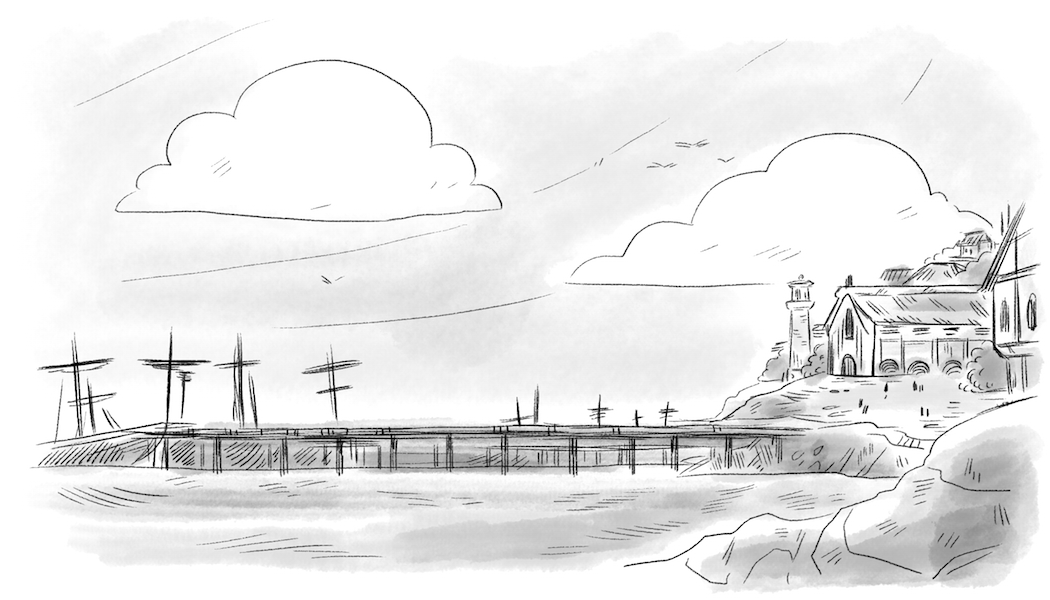
\includegraphics{img/port_of_goodnews.png}
  \caption{}
  \end{figure}
  
  Captain Z stared at the decoded message, trying to grasp its full
  meaning.
  
  A war? A battle, with pirates? That couldn't be right. She must have
  made a mistake.
  
  The Port of Goodnews was one of the most guarded cities in all the
  Western Waters. It was small, compared to some of the cities of the
  Eastern Coast, but still had more guards and galleys than many of them.
  Certainly no pirate would be dumb enough to attack the city outright.
  
  Still, the message filled Captain Z with dread. It was now Friday
  morning. In an hour or so, the sun would begin to rise on a new day.
  
  She listened for any strange sounds outside. If pirates were planning an
  attack, they would have been spotted by now. Guards would be running to
  their stations. Alarms would be going off. Captain Z listened, but heard
  nothing. Everything outside was quiet and peaceful, to be expected at
  this early hour.
  
  Just to make sure, the captain decided to take a quick look around
  outside. She wanted to get a good look at the harbor from above.
  
  Captain Z crept out of the school and up the alley. She turned the
  corner and started up the bumpy hill to Lookout Point. Street after
  street, she looked down as she jogged past and saw nothing but dark
  homes. A few times she turned around to try to see the harbor, but trees
  and smaller hills blocked the view.
  
  The sky was starting to light up just a bit when she found the path to
  the viewing spot. She ran down the path and onto the lookout's little
  platform. There she could see all the harbor at once.
  
  What she saw took her breath away.
  
  In the dim light, Captain Z could see what looked to be an entire fleet
  of ships filling the harbor. Many of them looked to be flying the black
  flag of the Jolly Roger. Pirates had invaded the port.
  
  Most were floating out in the open waters, in a loose formation. A few
  were docking near the center of town. From where she stood, high up on
  the hill, Captain Z could barely make out pirate crews coming off these
  docked ships. They were coming into the city and moving between the
  docked boats on the piers.
  
  Amazingly, the town guard and its fleet where nowhere to be seen.
  \emph{Something bad must have happened,} she thought. \emph{The guards
  would not simply sleep through such an invasion.}
  
  She thought back to the market chase and Walter's warning about the
  guards. \emph{Perhaps the guards aren't guarding these people anymore,}
  she considered.
  
  Captain Z could just make out Wind Drinker in the dark. It sat where she
  had docked, on the far end of of the harbor. From what she could see,
  none of the pirates had tied up over there. At least, not yet.
  
  She couldn't see Muddle, but guessed she was still on the ship.
  
  Captain Z started running as fast as she could back down the hill. She
  had to warn Dr.~Star. And after that, she had to escape from Port
  Goodnews before the pirates started attacking. She loved a good fight,
  but was in no mood for a battle that she couldn't win. A pirate army
  against a sleeping town didn't sound like a fun time to her.
  
  \section{}\label{section-37}
  
  She made it back down to the school and slammed through the door.
  Captain Z ran through the hallway, pounding on the children's door to
  get them moving, before knocking on the door to Dr.~Star's room.
  
  Dr.~Star had heard Captain Z, as she came banging through the hall, and
  was sitting up in her bed when Sophia burst in.
  
  \enquote{I've decoded the message,} Captain Z said. She was out of
  breath from the long run. \enquote{Pirates are going to attack Port
  Goodnews this morning. Its a war.}
  
  Dr.~Star checked her watch. \enquote{Attack Goodnews? Are you sure the
  message is right?} She asked.
  
  \enquote{There is a whole fleet of pirate ships in the bay, right now.
  Some are coming into the town. The town guard is missing, or worse,
  joined with the pirates.}
  
  Dr.~Star's face became more serious with each word.
  
  \enquote{You have to get yourself and the children out of town,} Captain
  Z said firmly. \enquote{Who knows what these pirates plans are. If you
  leave now, you can make it.}
  
  \enquote{I wouldn't be able to make it out of here before they attacked,
  even if I left now,} Dr.~Star respond, shaking her head. \enquote{Plus,
  if a battle is coming, I need to be here to help the hurt and wounded.}
  
  It was true that there were few healers in the Port of Goodnews, and
  none were as skilled as Dr.~Star. \emph{But that doesn't mean she should
  stay and risk her life,} thought Captain Z.
  
  \enquote{If you take them now,} Dr.~Star suggested, \enquote{you could
  make it out fast enough to escape.}
  
  Captain Z was definitely planning on leaving now, or as close to now as
  possible. But she had no mind to be taking children along for the ride.
  
  She was about to argue about the idea, when she remembered the poem that
  came with the Pegasus feathers. She remembered the part about a hero
  being born. Perhaps she could be a pirate and a hero at the same time.
  
  Before she could respond, there was a knock at the bedroom door. Nova,
  Orion, and Lucy shuffled in.
  
  \enquote{What's going on?} Asked Nova.
  
  Captain Z didn't have time to explain. \enquote{You've got two minutes
  to change your clothes and pack your bag,} she answered. \enquote{You
  are leaving the city now, one way or another.}
  
  The children knew better then to ask questions of a pirate. They all ran
  out back out of the hallway to their room.
  
  \emph{Lucy might need a bit of help from Nova,} Captain Z thought.
  \emph{But they'll be ready to go.}
  
  \enquote{They would just slow me down,} Captain Z continued finally. But
  Dr.~Star could tell she was ready to take them. \enquote{With those
  brats, I might not get very far.}
  
  \enquote{They are quick on their feet, and quicker to learn,} Dr.~Star
  said. \enquote{Besides, I think luck will be on your side.}
  
  Captain Z glared at the doctor for a few seconds before storming off
  into her room to get ready. She knew she couldn't refuse such a request
  from Dr.~Star, but that didn't make it any easier.
  
  \section{}\label{section-38}
  
  Less then five minutes later, Captain Z and the three children were out
  of the house and down the block at the end of the alley.
  
  They went slow, peeking around corners and crouching as they passed the
  homes and shops on the way down the long hill toward the port. The piers
  were situated near the center of town. There would be plenty of places
  to hide as they went, as long as they were careful.
  
  Closer to the water, they started catching glimpses of groups of pirates
  heading this way and that. They all looked to be on a mission and not
  one was looking about to see Captain Z or her soon-to-be shipmates.
  
  Once they made it to the center of town, they crept down toward the far
  end of the piers where Wind Drinker was docked. They kept behind
  buildings and dry docked ships, so the pirates wouldn't see them coming.
  
  As they moved through the buildings, they saw glimpses of the boats
  docked along the piers. Pirates were surrounding some of the larger
  ships. Captain Z couldn't tell what those pirates were up to, but she
  knew it couldn't be something good.
  
  Finally, they made it to the far end of the harbor. They were hidden
  behind a boat house in front of the docks. The sky was getting lighter.
  The captain was surprised that the pirates hadn't started their attack
  yet. \emph{They must be waiting for some sort of signal,} she thought.
  
  From the pier, she begin to hear a familiar sound that put her on edge.
  Muddle was cawing wildly.
  
  The crew ran to the other side of the boat house to get closer to the
  ship.
  
  Peaking around the corner of the building, they looked down the pier
  toward Wind Drinker. Two pirates had untied the boat and were pulling it
  away from the dock. It looked as if they meant to drag it out to the bay
  so no one could board it. They would have finished their job by now if
  it weren't for Muddle.
  
  The crow was cawing and diving down at the pirates. With each swoop, she
  tried to peck at their hands or heads. The two pirates were ducking down
  and waving their arms, trying to scare off their attacker. Captain Z
  jumped out from behind the boathouse, charging down the dock toward her
  boat.
  
  The first pirate stood up as the captain met her. Before he could react,
  she had smashed into him with her shoulder. He flew backwards and off
  the dock, splashing into the water.
  
  The other pirate stood up and started shouting, \enquote{Zephyr's here!
  Zephyr's here!} Pirates from the other piers heard him calling and
  started running toward them.
  
  As he shouted, Muddle swooped again and beaked him hard on the top of
  his head. The pirate raised both hands to cover his head and shouted out
  in pain.
  
  Captain Z took advantage of the situation. She ran into the pirate as he
  held held his head. Giving him a hard shove, he stumbled and fell back
  into the cold water.
  
  The children ran down the pier to join Captain Z on the ship. More
  pirates reached the pier. Their boots pounded on the wooden planks as
  they ran.
  
  The captain pushed hard to get the boat away from the dock and then
  jumped aboard herself. She was loosing the main sail as the pirates
  reached them.
  
  \section{}\label{section-39}
  
  They were lucky to have a small boat. And lucky Captain Z had the
  riggings on cranks and pulleys.
  
  They were luckier still to have a steady wind blowing away from the town
  out toward the bay.
  
  With the main sail out, and the wind up, the ship quickly shifted away
  from the dock.
  
  It was ten feet away when the pirates made it to the end of the pier.
  One of the first tried to jump aboard, but came up short. It was further
  away then he expected, and he splashed into the water. He bobbed up and
  down in the water, spitting up water as he went.
  
  Other pirates ran to the edge but could only watch as the ship drifted
  further out. They shouted a few choice words but could do nothing from
  the land.
  
  The pirate ships in the bay were a different story though. Captain Z
  would need even more luck to get around them to escape the port.
  
  All of Wind Drinker's sails were out now. They picked up speed and cut
  through the calm waters, making an arc out toward the bay's entrance.
  The land formed a crescent around the water, with a narrow opening out
  to the ocean. On either side of the opening stood a guard tower, one for
  each peninsula.
  
  \emph{If the guards were turn coats,} the captain thought, \emph{we
  could get blown out of the water from the cannons in those towers.}
  
  Even if the towers were empty, the waterway between the two strips of
  land could be easily blocked by a ship or two. If the pirates moved to
  trap them in, Wind Drinker would be stuck in a very small bit of water
  with all these angry pirates.
  
  But at first, none of the other ships moved to stop them. The pirates
  didn't want to break formation, they seemed afraid to get off track.
  
  \emph{Perhaps they are afraid any noise might wake the town and spoil
  their surprise,} Captain Z thought.
  
  Commotion or no, the town would be awake soon anyways. The sky was
  brighter now. The day was coming.
  
  Wind Drinker steered around two small pirate ships that were floating
  close to the piers. The captain and the children stared into the faces
  of the pirates aboard the nearest one. They were all glaring at the
  runaway ship, but weren't moving to stop it. Every few seconds they
  would look back toward the entrance to the port, as if expecting a
  signal of some sort.
  
  Wind Drinker was half way to freedom when that signal came.
  
  A shot rang out from a large ship near the East peninsula. Then the
  bright light of a flare slowly arced its way over the waters.
  
  The pirates sprang into action. Captains on all the ships started
  barking orders to their men. A few seconds later, the first booms of
  cannons could be heard. They were firing into the town!
  
  The sleeping townspeople didn't know it, but the war had begun.
  
  \section{}\label{section-40}
  
  As Captain Zephyr had been sneaking towards her boat, Captain Spears was
  already on his. Waiting for the signal like all the other pirates in the
  bay who had made a pact with the leader behind this sinister plan.
  
  He had put his boat, the Sea Breaker, far out in the waters, near the
  port's entrance. He hoped to avoid most of the action.
  
  Spears had agreed to join the battle against the Port of Goodnews, not
  because he wanted to capture the city, but because he feared what would
  happen to him if he refused. The whole ordeal left a sour taste in his
  mouth. \emph{Waiting in the water like eels in the dark,} he thought,
  \emph{it doesn't seem right.}
  
  As they say, a fight is no fun if your match doesn't know they are
  fighting.
  
  Still, he was there waiting in the dark, just the same.
  
  \begin{figure}[htbp]
  \centering
  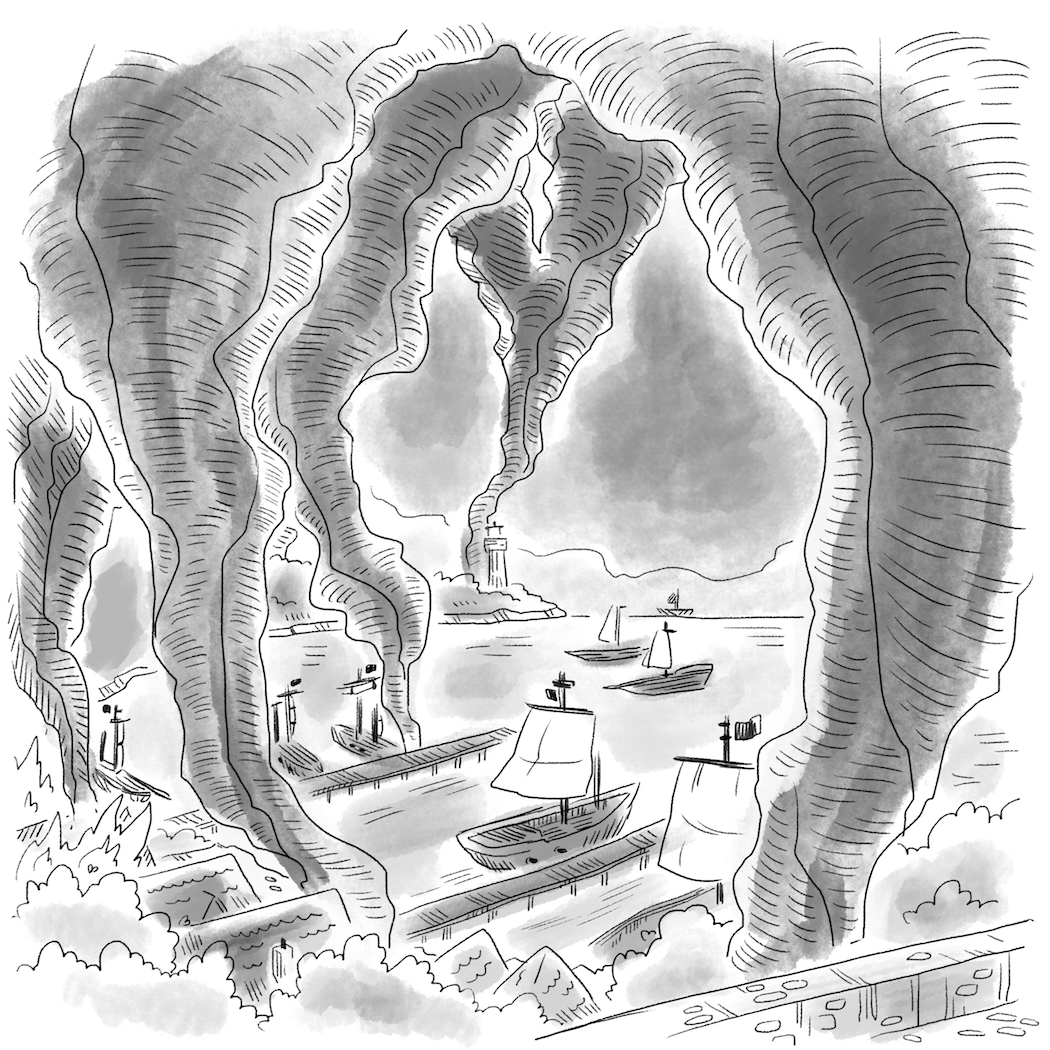
\includegraphics{img/battle_of_the_port.png}
  \caption{}
  \end{figure}
  
  As he was thinking about this, he heard strange noises coming from far
  off on the shore. He turned to gaze out with his red eye to see what was
  going on. The eye focused on a big black bird, a crow. The same crow he
  had seen on Castle Island! It was screeching and diving at pirates on
  the pier near a familar looking boat.
  
  His eye lit up at the sight of the bird. \emph{What is that thing doing
  in Goodnews?} Spears wondered. \emph{It should be still mourning the
  loss of its poor little captain out on Castle Island.}
  
  Then, he saw Captain Zephyr herself running down the pier toward her
  ship. Captain Spears nearly fell overboard from the sight. She was
  alive!
  
  \enquote{Well I'll be a talkin' gator,} he said to himself.
  
  She was far off, but his red eye made sure it was her. The eye was
  glowing hot now, like an iron just out of the fire.
  
  She should be dead, but wasn't. Which meant that perhaps the lost
  treasure of Castle Island wasn't really lost either.
  
  Then the flare shot up from the leaders boat. The signal to start the
  invasion.
  
  Captain Spears watched it as it lit the sky red over the water. He saw
  the other captains dutifully follow their orders to start the attack.
  But Captain Spears now had another reason not to join in the battle. If
  he could block Wind Drinker from leaving the bay, perhaps he could get
  his hands on the treasure Captain Zephyr had stolen.
  
  He spoke in a hushed voice to his crew to explain the plan. Then he gave
  the order and the Sea Breaker started slowly making its way toward the
  entrance to the bay.
  
  If Captain Zephyr wanted out, she would have to get through Spears and
  the Sea Breaker.
  
  \section{}\label{section-41}
  
  With all the commotion, most of the attackers didn't even notice Wind
  Drinker sprinting out of the port. But one of the two ships Captain Z
  passed started to give chase. They pulled their sails around to turn and
  follow Captain Z as she steered away from the pier.
  
  It was Captain Pete Moss on the ship following Wind Drinker. Captain Z
  recognized him as they pulled in behind.
  
  Captain Moss had a slow ship and a slower crew. They were weighted down
  with a slew of cannons he was itching to use. And he would have used
  them on Wind Drinker if the port hadn't been so crowded with other
  pirate ships. One missed shot and he could sink an attacking ship.
  
  So, Captain Moss trailed behind Captain Z's ship as it weaved to and fro
  between the other ships in the harbor. Captain Z took her ship wide
  around the pirate swarm to stay clear of the cannons firing into the
  city.
  
  Even from a distance, the cannon blasts were loud and scary. Lucy hid at
  the back of the boat and covered her ears. Orion and Nova kept their
  heads up, but ducked down with every nearby blast.
  
  Captain Moss was not a skilled sailor, nor was his crew accustom to
  taking orders. They all had spent the last year living the land lovers
  life in Bodega. Now out in the water again, the crew had lost their sea
  legs.
  
  So when Zephyr cut sharply through the water around a big galley, Pete
  Moss didn't follow, though he tried. Shouting to the crew to tack in the
  sails and turning the wheel as hard as he could, his barge started into
  the turn. But the ropes on the sails were tangled and twisted up and his
  big boat couldn't turn sharp enough.
  
  The front side of his ship smashed into the back half of the galley with
  a deafening screech. Moss's ship took all the damage. It lurched to a
  stop, sending the Captain and his crew flying to the deck floor. Planks
  and other bits of wood were thrown across the water. Moss got up to look
  at the front of his boat to find a huge gash where sea water was
  flooding in.
  
  Moss started shouting to abandon ship, and within seconds he and his
  crew were lowering their rowboats into the water. The pirates started
  rowing as fast as they could while their ship tipped sideways into the
  water.
  
  The ship sank completely into the water a few minutes later. Captain
  Moss and his crew watched it go down, then sadly rowed for shore.
  
  The crew on the galley that had been hit watched them from their deck,
  making sure to note all the pirates involved in the disaster. The leader
  would hear about this.
  
  Zephyr sailed on.
  
  With all the other pirates focused on the town, or the crash, it looked
  like the way was clear for them to escape.
  
  Captain Z pulled Wind Drinker around to point directly at the entrance
  to the bay. It was still open, and free of ships. Despite the cannon
  fire and the commotion all around, Captain Z smiled at her luck.
  \emph{We made it,} she thought.
  
  That's when she saw the Sea Breaker slowly maneuvering through the
  waters towards the entrance. Captain Z's hear was gripped with fear.
  Spears had seen her, and was going to cut them off before they made it
  out!
  
  \section{}\label{section-42}
  
  Captain Z panicked. The Sea Breaker was big enough to block much of
  their way out. Wind Drinker could probably dodge around it, but then
  they would be in open water. Out there, with no other ships around,
  Captain Spears would be free to blast away with his cannons. Captain Z
  knew her ship couldn't stand up to that kind of fire power. They would
  be helpless if Spears attacked. The game would be up.
  
  If Spears and his crew boarded the ship, Captain Z would most likely be
  held captive. The children would be prisoners in the Port of Goodnews,
  with no one to protect them. And the feathers would be stolen.
  
  The feathers!
  
  Captain Z had forgotten her treasure, but now she wondered if they might
  be her one chance out.
  
  \emph{What if Wind Drinker is my steed?} She wondered. There was only
  one way to find out.
  
  She roped the wheel steady so that it stayed on course. They were still
  headed right for the entrance to the bay. The Sea Breaker was reaching
  the entrance already. It slowed near the western edge of the entrance.
  
  Captain Z pulled the feathers out of her pocket and looked them over.
  Then she slowly touched them to the ship's wheel.
  
  Nothing happened.
  
  She didn't loose hope. Moving to the front deck, she tried the floor,
  the railing, and even the main mast. She touched the feather to each
  spot hoping for some magic to happen. But the feathers did nothing, and
  the ship remained in the water.
  
  Lucy, Orion, and Nova watched Captain Z frantically move about the ship,
  jamming the feathers here and there. They could feel the fear rising in
  their bellies. Even Muddle above started to caw with fear.
  
  Captain Spears had positioned his ship along the edge of the entrance to
  the port. The crew started loading grape shot and mast breakers into
  their cannons. As Wind Drinker passed by, they would fire the shots and
  blast down the sails. Captain Z's ship would have no way to move and the
  treasure would be as good as gotten.
  
  Captain Z, now desperate, ran around the whole ship from front to back
  with two of the feathers in each hand, trying to get her steed up in the
  air. Finally, she stopped and cried out in frustration.
  
  Lucy looked up and uncovered her ears. She had an idea. In her loudest
  voice, she shouted to Captain Z over the commotion in the bay.
  
  \enquote{Try it on the wings!}
  
  Captain Z was confused until she saw that Lucy was pointing up. Captain
  Z looked up as well to see the sails of her ship blowing in the wind.
  \emph{The sails,} she thought, \emph{of course!}
  
  Filled out and full of air, the sails did look a bit like wings. Just
  like the Pegasus of legend, perhaps the feathers would work as part of
  the wings of the steed.
  
  \section{}\label{section-43}
  
  It was their last chance. Wind Drinker was almost alongside the Sea
  Breaker as it sped toward the entrance to the port. As soon as they were
  in range, Captain Spears would open fire.
  
  Captain Z ran to the mast and started climbing up the rope ladder to the
  sail. As she held on with one hand, she took two of the feathers in the
  other hand and jammed them into the sail cloth. The quill of one of the
  feathers stuck.
  
  Instantly, the boat jolted. The hull creaked loudly and lifted up
  partway out of the water.
  
  It worked! They were starting to float, but it wasn't enough. They were
  only a few feet out of the water.
  
  The jolt threw Captain Z back and she swung away holding on to the
  ladder. She swung herself back toward the sail and jabbed in the second
  feather.
  
  The ship creaked again as it lifted up completely out of the water. Now
  they were skimming across the surface of the sea, and they were moving
  at a breakneck speed.
  
  In two seconds, they would skim right in front of the Sea Breaker.
  
  \begin{figure}[htbp]
  \centering
  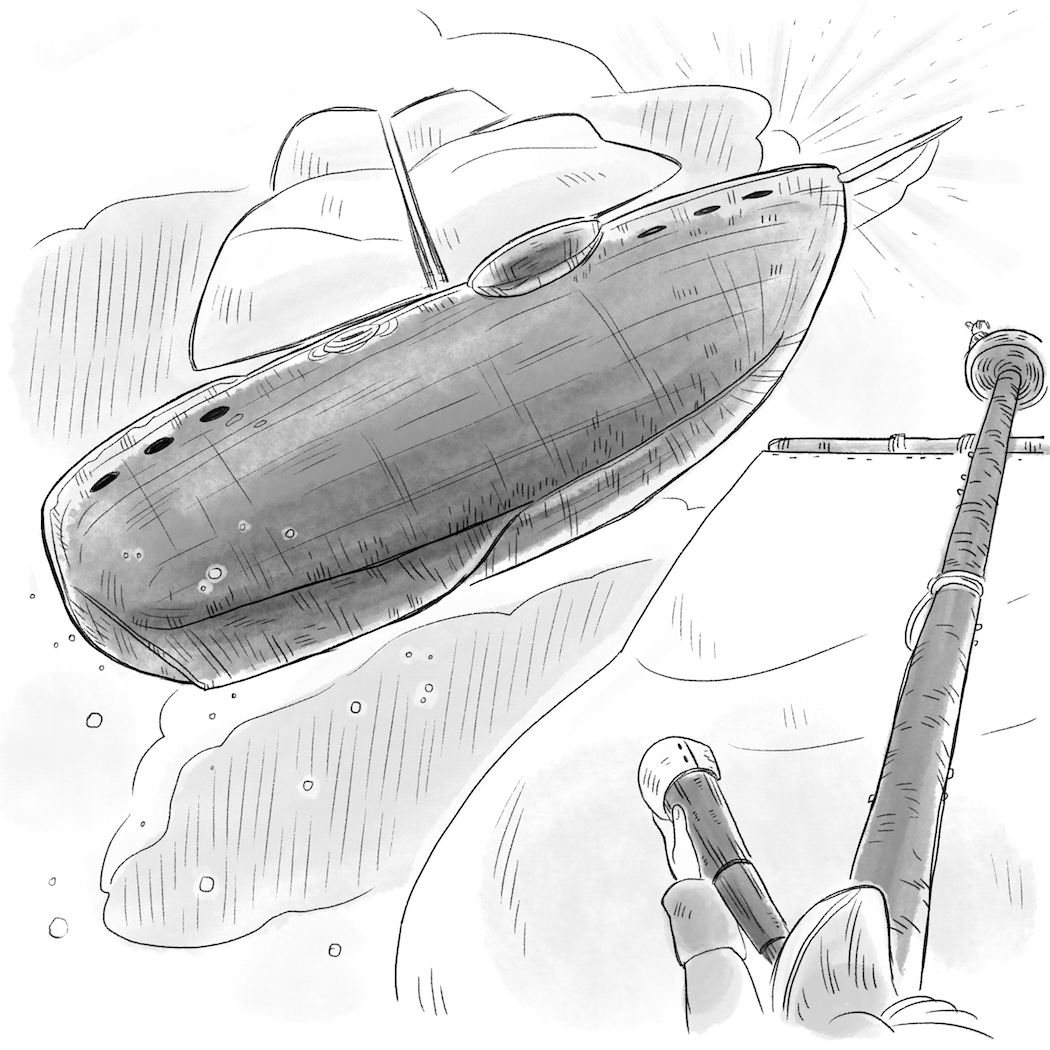
\includegraphics{img/flying_ship.png}
  \caption{}
  \end{figure}
  
  Desperately, Captain Z grabbed the last two feathers in her free hand
  and jumped up into the sail. Both feathers stuck to the sail as Captain
  Z fell down to the ground.
  
  Wind Drinker lurched into the air like a wind powered rocket.
  
  Captain Spears and his crew stood slack-jawed and silent. Their necks
  craned up as Captain Z's ship sailed over their heads and out towards
  the sea. No one could speak. Spears's eye changed to a brilliant yellow
  as he watched the flying vessel, not believing what he was seeing.
  
  Wind Drinker flew steadily up and up until finally leveling off high in
  the sky. Muddle flew along next to Captain Z and weaved back and forth
  among the masts deck as they went. The children began to cheer when they
  realized they had somehow escaped.
  
  Captain Z lashed the feathers to the sail with a bit of string and
  jumped down to join in the celebration.
  
  With no water to slow it down, the ship flew as fast as the wind. The
  Sea Breaker was soon just a small dot on the horizon. \emph{But how do I
  steer?} Captain Z wondered. Without water to push around, a rudder
  should be of no use. She decided to try the wheel anyways, just to be
  sure. She untied the ropes that were keeping it steady and slowly
  started to turn it.
  
  Magically, the ship started to turn as well! The movement was faster
  than what you would expect in the water, but that was no problem for
  Captain Z. She would learn to fly the ship just as well as she could
  sail it.
  
  \section{}\label{section-44}
  
  The cheering stopped as the children turned to look back to see a
  glimpse of the destruction of the Port of Goodnews. It was far off now
  in the distance now, but they could still make out smoke and fire coming
  from the buildings near the bay. The pirates were no doubt taking the
  city for themselves.
  
  \enquote{The people need our help,} Nova said.
  
  \enquote{They need help, Aye,} Captain Z said. \enquote{But one ship
  won't do a lick of good, even one that flys.} She turned to look at Nova
  and the other two children that she had sworn to protect. \enquote{We
  can't save Goodnews, least not by ourselves.}
  
  Nova looked sad. \enquote{Then where do we go to get help?} She asked.
  
  Captain Z looked out over the water at the breathtaking sunrise. The sky
  glowed orange and red, and the clouds were fringed in purple. She turned
  the wheel and pointed the ship directly toward the great ball of light.
  
  \enquote{East,} the captain replied.
  
  No one in the Western Waters was strong enough to fight back a pirate
  crew that could take Port Goodnews. If what the note said was true, that
  this was a war and not just one fight, then this morning's attack was
  only the beginning of something much bigger.
  
  The Eastern Coast would be their only hope for finding help. The armies
  there could march down and put a quick end to any pirate uprising.
  \emph{If they believe us,} Captain Z thought, \emph{and if they agree to
  help.}
  
  Getting there was a long trip by sea, but to fly would be a different
  story. \emph{As long as the wind blows strong, we might get there in
  time,} Captain Z thought. It would still be a tough trek, one Captain Z
  had never tried before, though she knew the way. They would have to make
  it over the Porter mountains and then through the Casperian desert.
  
  Orion, Nova, and Lucy walked over next to their captain to squint into
  the sunrise and look out. They would need to learn quickly how to help
  aboard Wind Drinker and work together if the plan was to be a success.
  
  Lucy was thinking about something and frowned as she looked up at
  Captain Z.
  
  \enquote{So, are we pirates now?} She asked. She knew Captain Z called
  herself a pirate, and that was fine, but otherwise, she wasn't very fond
  of any pirates that she knew of. She didn't want to have to be a pirate,
  if she didn't have to.
  
  \enquote{Not pirates,} Captain Z said. \enquote{That name's a bad fit.}
  
  \emph{But then what are we?} The captain thought.
  
  \enquote{Adventurers!} Nova shouted, as if reading her mind.
  
  Captain Z thought the name over in her head, then nodded her head yes.
  \emph{Adventurer suits me well,} she thought. She was tired of playing
  by pirate rules anyways. They would make up new rules as they went
  along.
  
  \enquote{Captain Z and the Adventurers,} Nova said again, and smiled.
  
  As Captain Z returned to the ship's wheel, her mind turned to all those
  pirates in the Port of Goodnews, and who could be the leader of such a
  crew. \emph{Who's cruel enough and powerful enough to make that many
  pirates fight together?} She wondered. Certainly not Captain Spears. He
  was greedy, to be certain, but he would never want a whole town to call
  his own. And he certainly didn't have enough smarts to make a plan like
  that work.
  
  No. Someone far more cruel was behind this war. Controlling the pirates
  like pieces on a chessboard. It made Sophia's skin crawl just to think
  about someone that terrible.
  
  \emph{Whoever it is, we'll make him pay,} she decided.
  
  \section{}\label{section-45}
  
  So our hero, no longer a pirate, but part of a crew of adventurers,
  sailed through the blue skies of the Western Waters, heading east as
  fast as they could fly.
  
  Over the mountains and through the desert, they would find an army to
  fight for the people of Goodnews and others in the Western Waters. At
  least that was the plan.
  
  The Port of Goodnews would be captured no doubt by the pirates, probably
  even before the sun set on the day. And then whoever was leading those
  scoundrels would most likely turn their eyes to other nearby towns.
  Captain Z hoped that there would be few people hurt in the attacks. She
  hoped someone in the cities of the Eastern Coast would listen to their
  story and come to stop the invasion. The quicker they could find help
  and come back to fight, the better.
  
  Muddle swooped down to land on her perch near the captain's wheel. She
  kept her wings outstretched, letting the wind blow through them as she
  held on to the stand with her feet.
  
  Nova, Orion, and Lucy continued to stare out into the wide ocean they
  were travelling above. Soon enough they would need to get to work,
  learning the ins and outs of the ship and how to manage it. They would
  also need to chart the course they would take out to the Eastern Coast.
  But for now, Captain Z let them enjoy the view.
  
  This would be the beginning of their adventures.

\end{document}

